% Options for packages loaded elsewhere
\PassOptionsToPackage{unicode}{hyperref}
\PassOptionsToPackage{hyphens}{url}
\PassOptionsToPackage{dvipsnames,svgnames,x11names}{xcolor}
%
\documentclass[
  letterpaper,
  DIV=11,
  numbers=noendperiod]{scrartcl}

\usepackage{amsmath,amssymb}
\usepackage{iftex}
\ifPDFTeX
  \usepackage[T1]{fontenc}
  \usepackage[utf8]{inputenc}
  \usepackage{textcomp} % provide euro and other symbols
\else % if luatex or xetex
  \usepackage{unicode-math}
  \defaultfontfeatures{Scale=MatchLowercase}
  \defaultfontfeatures[\rmfamily]{Ligatures=TeX,Scale=1}
\fi
\usepackage{lmodern}
\ifPDFTeX\else  
    % xetex/luatex font selection
\fi
% Use upquote if available, for straight quotes in verbatim environments
\IfFileExists{upquote.sty}{\usepackage{upquote}}{}
\IfFileExists{microtype.sty}{% use microtype if available
  \usepackage[]{microtype}
  \UseMicrotypeSet[protrusion]{basicmath} % disable protrusion for tt fonts
}{}
\makeatletter
\@ifundefined{KOMAClassName}{% if non-KOMA class
  \IfFileExists{parskip.sty}{%
    \usepackage{parskip}
  }{% else
    \setlength{\parindent}{0pt}
    \setlength{\parskip}{6pt plus 2pt minus 1pt}}
}{% if KOMA class
  \KOMAoptions{parskip=half}}
\makeatother
\usepackage{xcolor}
\setlength{\emergencystretch}{3em} % prevent overfull lines
\setcounter{secnumdepth}{-\maxdimen} % remove section numbering
% Make \paragraph and \subparagraph free-standing
\ifx\paragraph\undefined\else
  \let\oldparagraph\paragraph
  \renewcommand{\paragraph}[1]{\oldparagraph{#1}\mbox{}}
\fi
\ifx\subparagraph\undefined\else
  \let\oldsubparagraph\subparagraph
  \renewcommand{\subparagraph}[1]{\oldsubparagraph{#1}\mbox{}}
\fi

\usepackage{color}
\usepackage{fancyvrb}
\newcommand{\VerbBar}{|}
\newcommand{\VERB}{\Verb[commandchars=\\\{\}]}
\DefineVerbatimEnvironment{Highlighting}{Verbatim}{commandchars=\\\{\}}
% Add ',fontsize=\small' for more characters per line
\usepackage{framed}
\definecolor{shadecolor}{RGB}{241,243,245}
\newenvironment{Shaded}{\begin{snugshade}}{\end{snugshade}}
\newcommand{\AlertTok}[1]{\textcolor[rgb]{0.68,0.00,0.00}{#1}}
\newcommand{\AnnotationTok}[1]{\textcolor[rgb]{0.37,0.37,0.37}{#1}}
\newcommand{\AttributeTok}[1]{\textcolor[rgb]{0.40,0.45,0.13}{#1}}
\newcommand{\BaseNTok}[1]{\textcolor[rgb]{0.68,0.00,0.00}{#1}}
\newcommand{\BuiltInTok}[1]{\textcolor[rgb]{0.00,0.23,0.31}{#1}}
\newcommand{\CharTok}[1]{\textcolor[rgb]{0.13,0.47,0.30}{#1}}
\newcommand{\CommentTok}[1]{\textcolor[rgb]{0.37,0.37,0.37}{#1}}
\newcommand{\CommentVarTok}[1]{\textcolor[rgb]{0.37,0.37,0.37}{\textit{#1}}}
\newcommand{\ConstantTok}[1]{\textcolor[rgb]{0.56,0.35,0.01}{#1}}
\newcommand{\ControlFlowTok}[1]{\textcolor[rgb]{0.00,0.23,0.31}{#1}}
\newcommand{\DataTypeTok}[1]{\textcolor[rgb]{0.68,0.00,0.00}{#1}}
\newcommand{\DecValTok}[1]{\textcolor[rgb]{0.68,0.00,0.00}{#1}}
\newcommand{\DocumentationTok}[1]{\textcolor[rgb]{0.37,0.37,0.37}{\textit{#1}}}
\newcommand{\ErrorTok}[1]{\textcolor[rgb]{0.68,0.00,0.00}{#1}}
\newcommand{\ExtensionTok}[1]{\textcolor[rgb]{0.00,0.23,0.31}{#1}}
\newcommand{\FloatTok}[1]{\textcolor[rgb]{0.68,0.00,0.00}{#1}}
\newcommand{\FunctionTok}[1]{\textcolor[rgb]{0.28,0.35,0.67}{#1}}
\newcommand{\ImportTok}[1]{\textcolor[rgb]{0.00,0.46,0.62}{#1}}
\newcommand{\InformationTok}[1]{\textcolor[rgb]{0.37,0.37,0.37}{#1}}
\newcommand{\KeywordTok}[1]{\textcolor[rgb]{0.00,0.23,0.31}{#1}}
\newcommand{\NormalTok}[1]{\textcolor[rgb]{0.00,0.23,0.31}{#1}}
\newcommand{\OperatorTok}[1]{\textcolor[rgb]{0.37,0.37,0.37}{#1}}
\newcommand{\OtherTok}[1]{\textcolor[rgb]{0.00,0.23,0.31}{#1}}
\newcommand{\PreprocessorTok}[1]{\textcolor[rgb]{0.68,0.00,0.00}{#1}}
\newcommand{\RegionMarkerTok}[1]{\textcolor[rgb]{0.00,0.23,0.31}{#1}}
\newcommand{\SpecialCharTok}[1]{\textcolor[rgb]{0.37,0.37,0.37}{#1}}
\newcommand{\SpecialStringTok}[1]{\textcolor[rgb]{0.13,0.47,0.30}{#1}}
\newcommand{\StringTok}[1]{\textcolor[rgb]{0.13,0.47,0.30}{#1}}
\newcommand{\VariableTok}[1]{\textcolor[rgb]{0.07,0.07,0.07}{#1}}
\newcommand{\VerbatimStringTok}[1]{\textcolor[rgb]{0.13,0.47,0.30}{#1}}
\newcommand{\WarningTok}[1]{\textcolor[rgb]{0.37,0.37,0.37}{\textit{#1}}}

\providecommand{\tightlist}{%
  \setlength{\itemsep}{0pt}\setlength{\parskip}{0pt}}\usepackage{longtable,booktabs,array}
\usepackage{calc} % for calculating minipage widths
% Correct order of tables after \paragraph or \subparagraph
\usepackage{etoolbox}
\makeatletter
\patchcmd\longtable{\par}{\if@noskipsec\mbox{}\fi\par}{}{}
\makeatother
% Allow footnotes in longtable head/foot
\IfFileExists{footnotehyper.sty}{\usepackage{footnotehyper}}{\usepackage{footnote}}
\makesavenoteenv{longtable}
\usepackage{graphicx}
\makeatletter
\def\maxwidth{\ifdim\Gin@nat@width>\linewidth\linewidth\else\Gin@nat@width\fi}
\def\maxheight{\ifdim\Gin@nat@height>\textheight\textheight\else\Gin@nat@height\fi}
\makeatother
% Scale images if necessary, so that they will not overflow the page
% margins by default, and it is still possible to overwrite the defaults
% using explicit options in \includegraphics[width, height, ...]{}
\setkeys{Gin}{width=\maxwidth,height=\maxheight,keepaspectratio}
% Set default figure placement to htbp
\makeatletter
\def\fps@figure{htbp}
\makeatother
% definitions for citeproc citations
\NewDocumentCommand\citeproctext{}{}
\NewDocumentCommand\citeproc{mm}{%
  \begingroup\def\citeproctext{#2}\cite{#1}\endgroup}
\makeatletter
 % allow citations to break across lines
 \let\@cite@ofmt\@firstofone
 % avoid brackets around text for \cite:
 \def\@biblabel#1{}
 \def\@cite#1#2{{#1\if@tempswa , #2\fi}}
\makeatother
\newlength{\cslhangindent}
\setlength{\cslhangindent}{1.5em}
\newlength{\csllabelwidth}
\setlength{\csllabelwidth}{3em}
\newenvironment{CSLReferences}[2] % #1 hanging-indent, #2 entry-spacing
 {\begin{list}{}{%
  \setlength{\itemindent}{0pt}
  \setlength{\leftmargin}{0pt}
  \setlength{\parsep}{0pt}
  % turn on hanging indent if param 1 is 1
  \ifodd #1
   \setlength{\leftmargin}{\cslhangindent}
   \setlength{\itemindent}{-1\cslhangindent}
  \fi
  % set entry spacing
  \setlength{\itemsep}{#2\baselineskip}}}
 {\end{list}}
\usepackage{calc}
\newcommand{\CSLBlock}[1]{\hfill\break\parbox[t]{\linewidth}{\strut\ignorespaces#1\strut}}
\newcommand{\CSLLeftMargin}[1]{\parbox[t]{\csllabelwidth}{\strut#1\strut}}
\newcommand{\CSLRightInline}[1]{\parbox[t]{\linewidth - \csllabelwidth}{\strut#1\strut}}
\newcommand{\CSLIndent}[1]{\hspace{\cslhangindent}#1}

\usepackage{booktabs}
\usepackage{longtable}
\usepackage{array}
\usepackage{multirow}
\usepackage{wrapfig}
\usepackage{float}
\usepackage{colortbl}
\usepackage{pdflscape}
\usepackage{tabu}
\usepackage{threeparttable}
\usepackage{threeparttablex}
\usepackage[normalem]{ulem}
\usepackage{makecell}
\usepackage{xcolor}
\KOMAoption{captions}{tableheading}
\usepackage{float}
\makeatletter
\@ifpackageloaded{caption}{}{\usepackage{caption}}
\AtBeginDocument{%
\ifdefined\contentsname
  \renewcommand*\contentsname{Table of contents}
\else
  \newcommand\contentsname{Table of contents}
\fi
\ifdefined\listfigurename
  \renewcommand*\listfigurename{List of Figures}
\else
  \newcommand\listfigurename{List of Figures}
\fi
\ifdefined\listtablename
  \renewcommand*\listtablename{List of Tables}
\else
  \newcommand\listtablename{List of Tables}
\fi
\ifdefined\figurename
  \renewcommand*\figurename{Figure}
\else
  \newcommand\figurename{Figure}
\fi
\ifdefined\tablename
  \renewcommand*\tablename{Table}
\else
  \newcommand\tablename{Table}
\fi
}
\@ifpackageloaded{float}{}{\usepackage{float}}
\floatstyle{ruled}
\@ifundefined{c@chapter}{\newfloat{codelisting}{h}{lop}}{\newfloat{codelisting}{h}{lop}[chapter]}
\floatname{codelisting}{Listing}
\newcommand*\listoflistings{\listof{codelisting}{List of Listings}}
\makeatother
\makeatletter
\makeatother
\makeatletter
\@ifpackageloaded{caption}{}{\usepackage{caption}}
\@ifpackageloaded{subcaption}{}{\usepackage{subcaption}}
\makeatother
\ifLuaTeX
  \usepackage{selnolig}  % disable illegal ligatures
\fi
\usepackage{bookmark}

\IfFileExists{xurl.sty}{\usepackage{xurl}}{} % add URL line breaks if available
\urlstyle{same} % disable monospaced font for URLs
\hypersetup{
  pdftitle={Exploring MLB Batting Data Using Logistic Regression},
  pdfauthor={Vivian Johnson},
  colorlinks=true,
  linkcolor={blue},
  filecolor={Maroon},
  citecolor={Blue},
  urlcolor={Blue},
  pdfcreator={LaTeX via pandoc}}

\title{Exploring MLB Batting Data Using Logistic Regression}
\author{Vivian Johnson}
\date{}

\begin{document}
\maketitle
\begin{abstract}
This project aims to study classification and its applications to Major
League Baseball (MLB) batting data. The goal is to develop a model that
is capable of classifying a hit based on various in-game metrics,
including release speed, launch angle, bat speed, and swing length. The
model development process incorporates different statistical techniques
such as K-means cluster analysis and decision trees to understand the
distributions of the data and how observations are being classified in
the multinomial model. Additionally, specific balancing techniques are
explored to address inherent bias and imbalance in the data for the
purpose of making more accuracte classifications.
\end{abstract}

\newpage

\setcounter{tocdepth}{4}
\tableofcontents

\newpage

\section{Introduction}\label{introduction}

Baseball is a competitive game that revolves around a defensive
(fielding) team and an offensive (hitting) team. The field is shaped
like a diamond, with each of the four corners representing first,
second, third, and home respectively. The game lasts nine innings, where
each inning is broken down into a top half (where one team hits and the
other is on defense) and a bottom half, where they switch. Each half
inning has three outs, and the objective of the hitting team is to score
runs while the fielding team attempts to stop them by getting outs.

The game begins when the pitcher on the defensive team throws the
baseball overhand from sixty feet to the batter, who tries to hit the
ball with their wooden bat from home plate to somewhere out of reach of
one of the eight other defensive players. Once the ball is hit, the
batter tries to reach as many bases as possible without getting out. The
winner at the end of the game is the team who scored the most runs.

For the purposes of this project, we look to analyze the different
mechanics that go into an at bat, and how those swing mechanics
differentiate based on what type of hit the batter gets. The diagram
below shows the set up of a baseball field, where all the defensive
players are positioned, as well as where the batter stands.

\begin{figure}[H]

{\centering 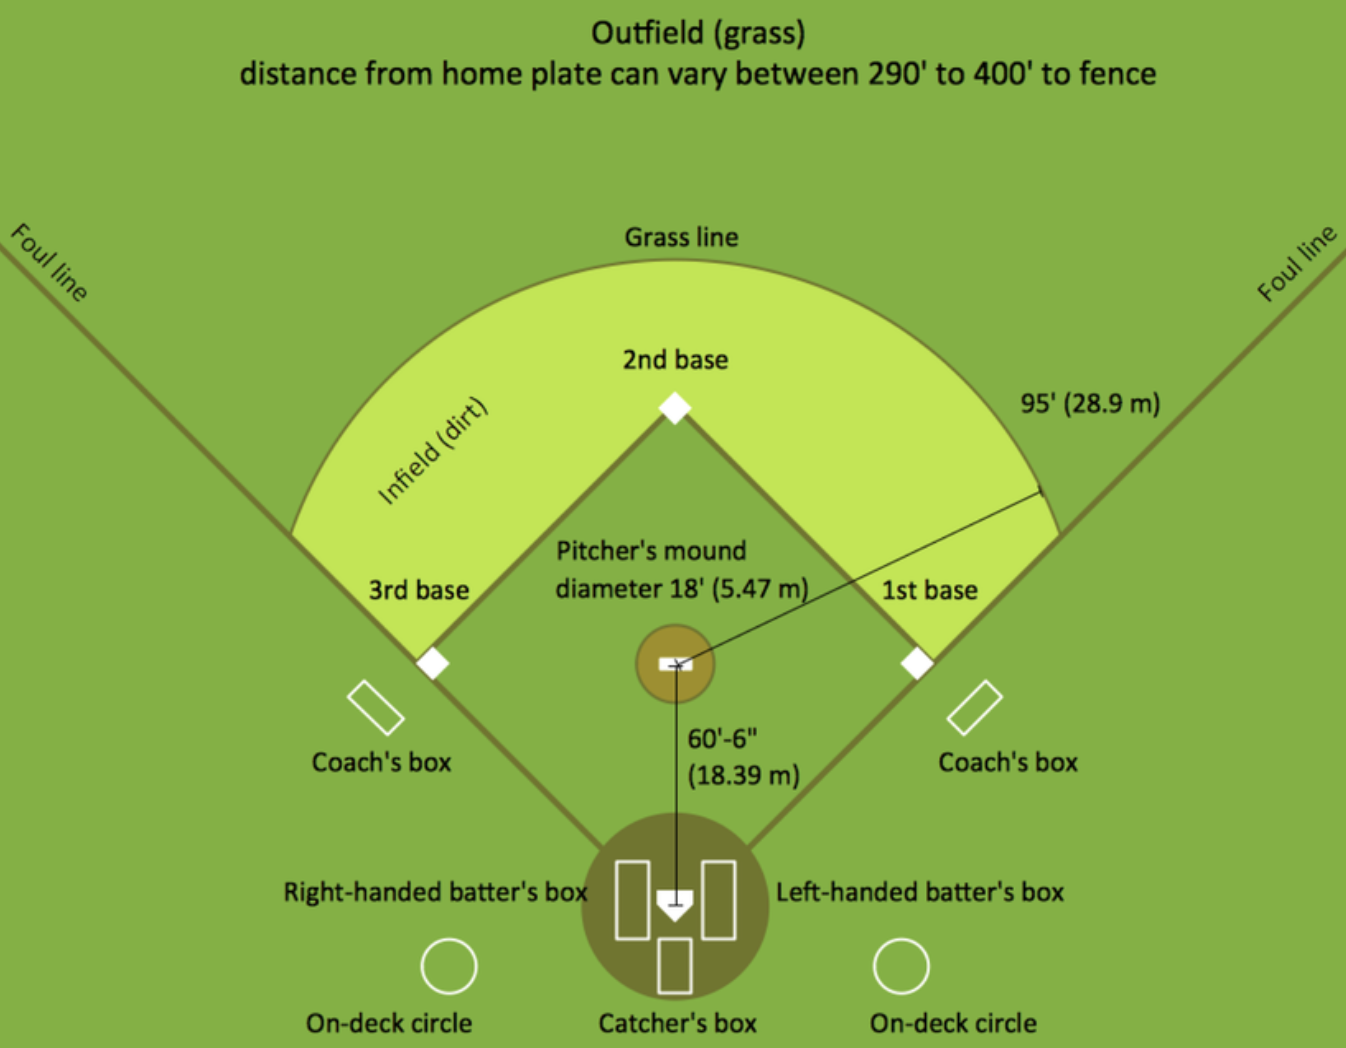
\includegraphics[width=0.8\textwidth,height=0.8\textheight]{baseball.png}

}

\caption{Diagram of baseball field (taken from
http://www.conceptdraw.com/solution-park/sport-baseball)}

\end{figure}%

\section{Important Baseball
Definitions}\label{important-baseball-definitions}

The terms below define key aspects of baseball that are relevant to this
project.

\begin{itemize}
\tightlist
\item
  \textbf{Ground Out:} The batter hits the ball on the ground, and the
  defensive player is able to throw the ball to first base before the
  batter gets there.
\item
  \textbf{Pop Fly/Out:} The batter hits the ball in the air, and a
  defensive player catches the ball without letting it touch the ground.
\item
  \textbf{Single:} A hit where the batter is able to make it safely to
  first base without stopping.
\item
  \textbf{Double:} A hit where the batter is able to make it safely to
  second base without stopping.
\item
  \textbf{Triple:} A hit where the batter is able to make it safely to
  third base without stopping.
\item
  \textbf{Homerun:} A hit where the batter is able to make it around
  every base and back to home without stopping, usually done by hitting
  the ball over the homerun fence, positioned about 350 feet, depending
  on the ballpark played at.
\end{itemize}

\section{Theory}\label{theory}

\subsection{Binary and Multinomial
Classification}\label{binary-and-multinomial-classification}

Classifying and predicting the type of hit that results from an at bat
can be described as a multinomial classification problem. Similar to
binary classification, where the response variable, Y, has two binary
categories, multinomial classification applies when there are multiple
possible event outcomes for Y. In this case, the possible results of the
hit are a single, double/triple (also referred to as an extra base hit),
or a homerun, encoded as 1, 2, or 3 respectively.

\subsection{Multinomial Logistic
Regression}\label{multinomial-logistic-regression}

When predicting a response variable with more than two (binary) levels,
the multinomial logistic regression model is effective. Similar to
regular logistic regression, the multinomial logistic regression model
predicts the probability of each level of Y.

In this case, for the dependent variable, \texttt{hit\_outcome}, we're
interested in looking at the probabilities of different hits occurring,
which can be written as \(P(Y=j)\). This includes singles, extra base
hits, and homeruns. Using multinomial logistic regression, this can be
modeled by the following equation:

\[P(Y=j | X_1 = x_1, X_2 = x_2, X_3 = x_3, X_4 = x_4, X_5 = x_5)\]
\[P(Y=j) = 
\frac{e^{\beta_0j + \beta_1jX_1 + \beta_2jX_2 + \beta_3jX_3 + \beta_4jX_4 + \beta_5jX_5}}{1 + \sum_{i = 1}^{j-1}{e^{\beta_0i + \beta_1iX_1 + \beta_2iX_2 + \beta_3iX_3 + \beta_4iX_4 + \beta_5iX_5}}}\]

Where \(X_1 ... X_5\) indicate the various predictor variables for the
multinomial logistic regression model. Since we're interested in the
probability of each hit given the different values of the five predictor
variables, we can transform the logit output from logistic regression to
the probability of the event occurring with the equation above.

\subsection{Accuracy, Precision, and Confusion
Matricies}\label{accuracy-precision-and-confusion-matricies}

To evaluate the performance of the multinomial logistic regression
model, a confusion matrix can be used and from that, the measures of
accuracy and precision can be found. A confusion matrix is a table that
shows for each value of the dependent variable, the number of true
positives and negatives, as well as the false positives and negatives.
In this case, as there are three levels of the dependent variable, the
confusion matrix is a 3x3 table.

For each specific class of the dependent variable:

\begin{itemize}
\tightlist
\item
  \textbf{True Positives (TP):} The number of observations that are
  correctly identified as being a part of that class.
\item
  \textbf{True Negatives (TN):} The number of observations that are
  correctly identified as not being a part of that class.
\item
  \textbf{False Positives (FP):} The number observations that are
  incorrectly identified as being a part of that class.
\item
  \textbf{False Negatives (FN):} The number of observations that are
  incorrectly identified as not being a part of that class.
\end{itemize}

From these metrics, accuracy (the accuracy in assigning the correct
categories to the data) can be defined as:

\[ Accuracy = \frac{TP + TN}{TP + FP + TN + FN}\]

As there are some disadvantages of accuracy with the raw initial data
set, precision can also be used to evaluate the model for each level of
the response variable (\(i\)). Precision is the ratio of true positives
to all observations that were identified as positives in the model.

\[Precision_i = \frac{TP_i}{TP_i + FP_i}\]

\section{Methods}\label{methods}

The data used in this project comes from Baseball Savant, the clearing
house for the Statcast data provided by the Major League Baseball
Association (MLB). The MLB employs advance statistical software and
sports tracking in order to keep various statistics throughout the
entirety of a major league game. Baseball Savant acts as the dashboard
through which the public can view and access the data straight from the
MLB (Statcast (2024)).

\subsection{Initial Data Preparation}\label{initial-data-preparation}

The data focuses on batting data from MLB games played from March 28,
2024 to October 30, 2024. The data was scraped from Baseball Savant
using the \texttt{statcast\_search()} function from the
\texttt{baseballr} package in R\footnote{Petti and Gilani (2024)}. Once
compiled, the data was saved to a CSV titled
\texttt{full\_batting\_data\_2024.csv}.

\begin{Shaded}
\begin{Highlighting}[]
\CommentTok{\# loading in the data }
\NormalTok{batting\_data\_2024 }\OtherTok{\textless{}{-}} \FunctionTok{read\_csv}\NormalTok{(}\StringTok{"season\_2024\_batting\_data.csv"}\NormalTok{)}
\end{Highlighting}
\end{Shaded}

\subsection{Data Cleaning}\label{data-cleaning}

The following code describes removing certain columns where data was no
longer collected and not useful to this project.

\begin{Shaded}
\begin{Highlighting}[]
\CommentTok{\# renaming certain columns }
\NormalTok{batting\_data\_2024 }\OtherTok{\textless{}{-}}\NormalTok{ batting\_data\_2024 }\SpecialCharTok{\%\textgreater{}\%}
  \FunctionTok{rename}\NormalTok{(}\AttributeTok{bat\_speed =}\NormalTok{ newStat\_1,}
         \AttributeTok{swing\_length =}\NormalTok{ newStat\_2)}

\CommentTok{\# removing deprecated columns }
\NormalTok{batting\_data\_2024 }\OtherTok{\textless{}{-}}\NormalTok{ batting\_data\_2024 }\SpecialCharTok{\%\textgreater{}\%}
  \FunctionTok{select}\NormalTok{(}\SpecialCharTok{{-}}\NormalTok{spin\_dir,}
         \SpecialCharTok{{-}}\NormalTok{spin\_rate\_deprecated,}
         \SpecialCharTok{{-}}\NormalTok{break\_angle\_deprecated,}
         \SpecialCharTok{{-}}\NormalTok{break\_length\_deprecated,}
         \SpecialCharTok{{-}}\NormalTok{tfs\_deprecated,}
         \SpecialCharTok{{-}}\NormalTok{tfs\_zulu\_deprecated,}
         \SpecialCharTok{{-}}\NormalTok{umpire}
\NormalTok{         )}
\end{Highlighting}
\end{Shaded}

\subsubsection{Important Variables}\label{important-variables}

Table~\ref{tbl-imp-variables} gives descriptions of the variables used
to create a model and analyze hit types.

\begin{table}

\caption{\label{tbl-imp-variables}Description of Important Variables
Used}

\centering{

\centering
\begin{tabular}[t]{>{\raggedright\arraybackslash}p{4cm}>{\raggedright\arraybackslash}p{7cm}}
\toprule
Variable & Description\\
\midrule
\cellcolor{gray!10}{events} & \cellcolor{gray!10}{Records the event of the resulting plate appearance (single, double, triple, homerun)}\\
release\_speed & The speed of the pitch that was thrown to the batter\\
\cellcolor{gray!10}{launch\_angle} & \cellcolor{gray!10}{Vertical launch angle of the batted ball as tracked by Statcast. Refers to the angle at which the ball leaves the bat}\\
bat\_speed & Measurement of how fast the bat is moving when the player makes contact with the ball\\
\cellcolor{gray!10}{swing\_length} & \cellcolor{gray!10}{Total amount of feet the bat traveled during the swing (the total distance traveled by the barrel of the bat in x/y/z space)}\\
\bottomrule
\end{tabular}

}

\end{table}%

\subsubsection{Indicator Variables}\label{indicator-variables}

The indicator variable \texttt{hit\_outcome} was created using the
\texttt{events} variable in the data set and serves as the dependent
variable for multinomial logistic regression. The table and code below
describe the variable, as well as creating it using the data and storing
it in an R object called \texttt{batting\_with\_indicators}.

\begin{Shaded}
\begin{Highlighting}[]
\CommentTok{\# making the indicator variables  }
\NormalTok{batting\_with\_indicators }\OtherTok{\textless{}{-}}\NormalTok{ batting\_data\_2024 }\SpecialCharTok{\%\textgreater{}\%} 
  \FunctionTok{filter}\NormalTok{(}
    \SpecialCharTok{!}\FunctionTok{is.na}\NormalTok{(bat\_speed) }\SpecialCharTok{\&}
      \SpecialCharTok{!}\FunctionTok{is.na}\NormalTok{(swing\_length) }\SpecialCharTok{\&}
      \SpecialCharTok{!}\FunctionTok{is.na}\NormalTok{(launch\_angle) }\SpecialCharTok{\&}
      \SpecialCharTok{!}\FunctionTok{is.na}\NormalTok{(release\_speed)}
\NormalTok{    ) }\SpecialCharTok{\%\textgreater{}\%}
  \FunctionTok{mutate}\NormalTok{(}
    \CommentTok{\# homerun variable: 1 if homerun, 0 if double }
    \AttributeTok{homerun =} \FunctionTok{case\_when}\NormalTok{(}
\NormalTok{      events }\SpecialCharTok{==} \StringTok{"home\_run"} \SpecialCharTok{\textasciitilde{}} \DecValTok{1}\NormalTok{,}
\NormalTok{      events }\SpecialCharTok{==} \StringTok{"double"} \SpecialCharTok{\textasciitilde{}} \DecValTok{0}\NormalTok{,}
      \ConstantTok{TRUE} \SpecialCharTok{\textasciitilde{}} \ConstantTok{NA\_real\_}\NormalTok{),}
    \CommentTok{\# hit\_outcome corresponds to the type of hit }
    \AttributeTok{hit\_outcome =} \FunctionTok{case\_when}\NormalTok{(}
\NormalTok{      events }\SpecialCharTok{==} \StringTok{"home\_run"} \SpecialCharTok{\textasciitilde{}} \DecValTok{3}\NormalTok{,}
\NormalTok{      events }\SpecialCharTok{==} \StringTok{"triple"} \SpecialCharTok{|}\NormalTok{ events }\SpecialCharTok{==} \StringTok{"double"} \SpecialCharTok{\textasciitilde{}} \DecValTok{2}\NormalTok{,}
\NormalTok{      events }\SpecialCharTok{==} \StringTok{"single"} \SpecialCharTok{\textasciitilde{}} \DecValTok{1}\NormalTok{)}
\NormalTok{    ) }\SpecialCharTok{\%\textgreater{}\%} \FunctionTok{filter}\NormalTok{(}
      \SpecialCharTok{!}\FunctionTok{is.na}\NormalTok{(hit\_outcome)}
\NormalTok{      )}
\end{Highlighting}
\end{Shaded}

\begin{table}

\caption{\label{tbl-indicator-variables}Description of Indicator
Variables Used}

\centering{

\centering
\begin{tabular}[t]{>{\raggedright\arraybackslash}p{4cm}>{\raggedright\arraybackslash}p{7cm}}
\toprule
Variable & Description\\
\midrule
\cellcolor{gray!10}{hit\_outcome} & \cellcolor{gray!10}{Indicator for the type of hit recorded in the `events` variable. 1 = single, 2 = extra base hit (double or triple), 3 = homerun}\\
\bottomrule
\end{tabular}

}

\end{table}%

\subsubsection{Standardizing Variables}\label{standardizing-variables}

The next step in cleaning the data was to standardize the
\texttt{swing\_length}, \texttt{bat\_speed}, \texttt{launch\_speed}, and
\texttt{release\_speed} variables.

Turning these variables into z-scores was done to normalize the data so
that each variable has a mean of zero and a standard deviation of one.
Therefore, an observation with a \texttt{swing\_length\_zscore} of 0.56
would indicate that that batter had a swing length 0.56 standard
deviations longer than the average swing length for all batters. This
process puts all observations for the variables on the same scale, and
aids in the interpretation of the regression models and comparison
across variables.

\begin{Shaded}
\begin{Highlighting}[]
\CommentTok{\# standardizing swing length, bat speed, and launch speed. }
\NormalTok{batting\_with\_indicators }\OtherTok{\textless{}{-}}\NormalTok{ batting\_with\_indicators }\SpecialCharTok{\%\textgreater{}\%}
  \FunctionTok{mutate}\NormalTok{(}
    \AttributeTok{swing\_length\_zscore =} \FunctionTok{scale}\NormalTok{(swing\_length),}
    \AttributeTok{bat\_speed\_zscore =} \FunctionTok{scale}\NormalTok{(bat\_speed),}
    \AttributeTok{release\_speed\_zscore =} \FunctionTok{scale}\NormalTok{(release\_speed)}
\NormalTok{  )}
\end{Highlighting}
\end{Shaded}

\subsection{Preliminary Data Analysis}\label{preliminary-data-analysis}

\subsubsection{Distributions of Independent
Variables}\label{distributions-of-independent-variables}

\begin{figure}[H]

\centering{

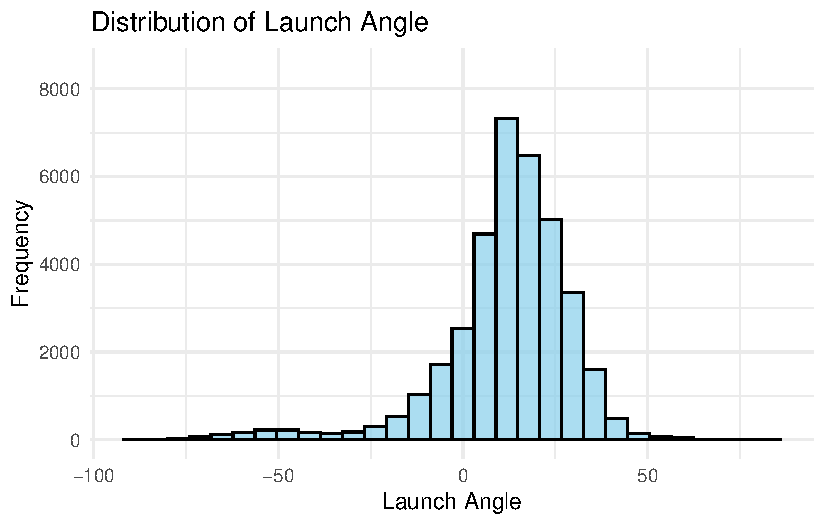
\includegraphics{V4_files/figure-pdf/fig-launch-angle-1.pdf}

}

\caption{\label{fig-launch-angle}Distribution of Launch Angle}

\end{figure}%

Figure~\ref{fig-launch-angle} above, and Figure~\ref{fig-dists} below,
show the distributions of the independent variables used during the
model development process. From these figures, we can see that all
follow an approximately normal distribution. Although multinomial
logistic regression does not require normally distributed independent
variables, this approximate normality could aid in interpretability.
Additionally, this normality suggests that transformations to the
independent variables such as log or polynomial terms might be
unnecessary.

\begin{figure}[H]

\centering{

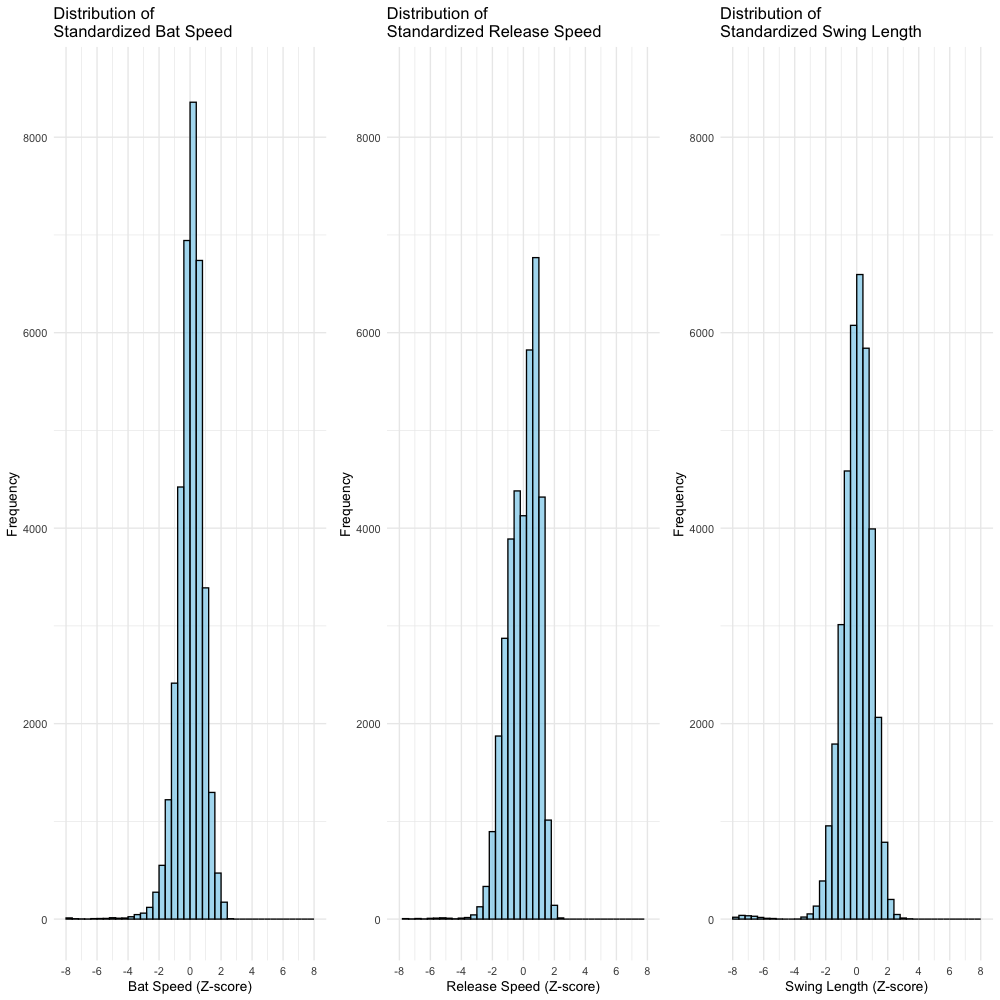
\includegraphics{combined_plots.png}

}

\caption{\label{fig-dists}Distributions of Standardized Independent
Variables}

\end{figure}%

\newpage

\subsubsection{Correlations}\label{correlations}

Table~\ref{tbl-corr} shows a correlation matrix for the independent
variables. The table includes standardized bat speed, standardized
release score, standardized swing length, and launch angle. The highest
correlation is between \texttt{bat\ speed} and \texttt{swing\ length},
with a value of \(0.589\). This indicates a moderate positive
correlation, which is logical, as higher bat speeds tend to be
associated with longer swing lengths.

Since this is the highest correlation, and other correlations are low,
multicollinearity does not appear to be a significant concern in the
data, given that none of the correlations are excessively high (above
0.8, which is usually considered to be an indicator of
multicollinearity).

\begin{table}

\caption{\label{tbl-corr}Correlation Matrix For Independent Varaibles}

\centering{

\centering
\begin{tabular}[t]{>{\raggedright\arraybackslash}p{2.5cm}>{\raggedleft\arraybackslash}p{2cm}>{\raggedleft\arraybackslash}p{2cm}>{\raggedleft\arraybackslash}p{2cm}>{\raggedleft\arraybackslash}p{2cm}}
\toprule
  & Bat Speed & Release Speed & Swing Length & Launch Angle\\
\midrule
\cellcolor{gray!10}{Bat Speed} & \cellcolor{gray!10}{1.000} & \cellcolor{gray!10}{0.011} & \cellcolor{gray!10}{0.589} & \cellcolor{gray!10}{0.174}\\
Release Speed & 0.011 & 1.000 & -0.256 & -0.045\\
\cellcolor{gray!10}{Swing Length} & \cellcolor{gray!10}{0.589} & \cellcolor{gray!10}{-0.256} & \cellcolor{gray!10}{1.000} & \cellcolor{gray!10}{0.148}\\
Launch Angle & 0.174 & -0.045 & 0.148 & 1.000\\
\bottomrule
\end{tabular}

}

\end{table}%

\subsubsection{K Means Cluster Analysis}\label{k-means-cluster-analysis}

\begin{figure}[H]

\centering{

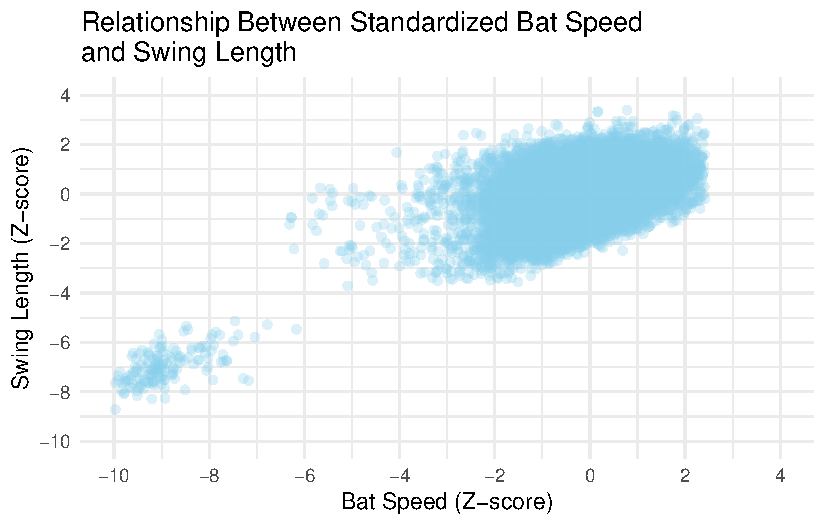
\includegraphics{V4_files/figure-pdf/fig-scatter1-1.pdf}

}

\caption{\label{fig-scatter1}Scatterplot of Bat Speed and Swing Length}

\end{figure}%

Figure~\ref{fig-scatter1} shows a moderately positive linear
relationship between the standardized swing length of a batter and the
standardized bat speed of the batter. From this, it can be understood
that longer swings tend to produce higher bat speeds. A reasoning for
this could be because with a longer bat path, the batter has more time
to generate speed in their swing. Due to this, it was decided to add an
interaction between bat speed and swing length, as the effect of bat
speed on hit outcome could also be affected by the batter's swing
length.

The scatterplot in Figure~\ref{fig-scatter1} also shows distinct
grouping within the data. There is a grouping of hits, most likely
bunts\footnote{A bunt is a strategic hit where the batter lightly taps
  the ball with the bat, usually to advance a runner already on base, or
  get on base quickly.} or soft ground balls, where the batters had much
lower swing lengths and bat speeds compared to the other observed hits.
To analyze this further, K-means cluster analysis was performed to look
at the specific groupings in the data.

K-Means Cluster Analysis is the process of grouping each observation in
the data based on distinct characteristics. Upon completion, groups will
be formed ideally with similar characteristics. The goal is to extract
relationships, in this case, between the swing length of the batter and
the bat speed. The algorithm begins by first determining how many groups
will be formed (K = 3 for this scenario). Then, 3 observations are
randomly chosen from the data, and assigned to a group. These rows act
as the preliminary centers (means) of the groups. The remaining
observations are individually assigned to the group that minimizes the
Euclidean distance\footnote{Euclidean distance is the straight line
  distance between two points in space.} between the observation and the
group mean. Following this, a new average for the groups are calculated,
and each observation is re-examined to see if it is closer to a
different groups average. This process repeats until no observation
changes groups. (Wu and Wu (2012))

The following code was used to perform the cluster analysis, while
Figure~\ref{fig-cluster} shows the corresponding groups that were
created.

\begin{Shaded}
\begin{Highlighting}[]
\CommentTok{\# selecting only the two columns needed}
\NormalTok{batting\_cluster }\OtherTok{\textless{}{-}}\NormalTok{ batting\_with\_indicators }\SpecialCharTok{\%\textgreater{}\%}
  \FunctionTok{select}\NormalTok{(swing\_length\_zscore,}
\NormalTok{         bat\_speed\_zscore)}

\FunctionTok{set.seed}\NormalTok{(}\DecValTok{12}\NormalTok{) }\CommentTok{\# so it is reproducible}
\NormalTok{cluster\_analysis }\OtherTok{\textless{}{-}} \FunctionTok{kmeans}\NormalTok{(batting\_cluster,}
                           \AttributeTok{centers =} \DecValTok{3}\NormalTok{,}
                           \AttributeTok{nstart =} \DecValTok{25}\NormalTok{)}
\end{Highlighting}
\end{Shaded}

\begin{figure}[H]

\centering{

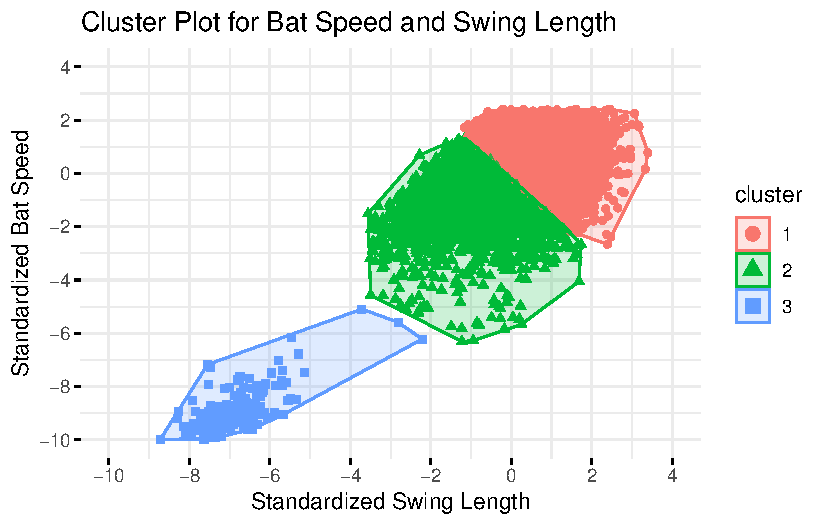
\includegraphics{V4_files/figure-pdf/fig-cluster-1.pdf}

}

\caption{\label{fig-cluster}Scatterplot showing clustered groups}

\end{figure}%

\begin{table}

\caption{\label{tbl-kmeanssum-variables}K-Means Summary Statistics}

\centering{

\centering
\begin{tabular}[t]{llll}
\toprule
Cluster & Cluster Size & Centers (swing length, bat speed) & WSS\\
\midrule
\cellcolor{gray!10}{1} & \cellcolor{gray!10}{21986} & \cellcolor{gray!10}{(0.559, 0.429)} & \cellcolor{gray!10}{15027}\\
2 & 14567 & (-0.767, -0.549) & 13916\\
\cellcolor{gray!10}{3} & \cellcolor{gray!10}{162} & \cellcolor{gray!10}{(-6.891, -8.857)} & \cellcolor{gray!10}{236}\\
\bottomrule
\end{tabular}

}

\end{table}%

Figure~\ref{fig-cluster} shows the results from performing K=3 Means
Cluster Analysis. It is evident that the third cluster has significantly
different bat speeds and swing lengths. Because the goal of this project
is to examine the difference in hitting mechanics between true singles,
extra base hits, and homeruns, it was determined that these hits, which
are most likely check swings or bunts, don't accurately represent the
data and that this cluster should be removed.

Table~\ref{tbl-kmeanssum-variables} describes the cluster size, center,
and within cluster sum of squares for each group. The within cluster sum
of squares, also known as the intra-cluster variation, is the sum of the
squared Euclidean distances between each observation and the center of
the cluster (Wu and Wu (2012)). A smaller WSS indicates that the
observations are grouped closer together, thus forming a more specific
group. Since the WSS of group 3 is significantly lower than the other
two groups and relatively small, removing the observations in this group
is not of high concern.

\begin{figure}[H]

\centering{

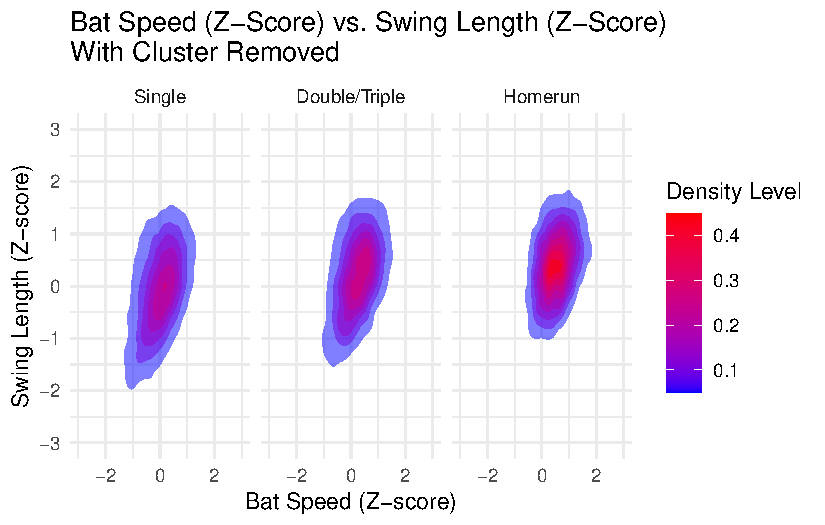
\includegraphics{V4_files/figure-pdf/fig-no-b-den-1.pdf}

}

\caption{\label{fig-no-b-den}The relationship between bat speed and
swing length for each hit outcome}

\end{figure}%

Figure~\ref{fig-no-b-den} shows the relationships between standardized
bat speed and standardized swing length for each level of
\texttt{hit\_outcome} after removing the cluster of hits. For each hit
outcome, there is a clear positive relationship between the bat speed
and the length of the swing. The density level represents how closely
packed the points are, (i.e.~where data points are more concentrated).
From Figure~\ref{fig-no-b-den}, we can see that the direction of the
relationship between the hit types are similar, but the densities and
variance differ. Homeruns vary the least, as the majority of the
observations that are homeruns are tightly concentrated. Singles tend to
vary the most, as there is not an extremely high density level anywhere
on the graph. This is somewhat logical, as there is more opportunity /
ways in which a batter could hit a potential single compared to a
homerun.

\subsubsection{Distributions Incorporating Ground Outs and Fly
Outs}\label{distributions-incorporating-ground-outs-and-fly-outs}

The data allows us to differentiate between fly outs and ground outs,
meaning that we can also observe the difference in the independent
variables between these types of outs, as well as hits. This is
important as it aids in understanding how these factors differ between
outs and hits.

\begin{figure}[H]

\centering{

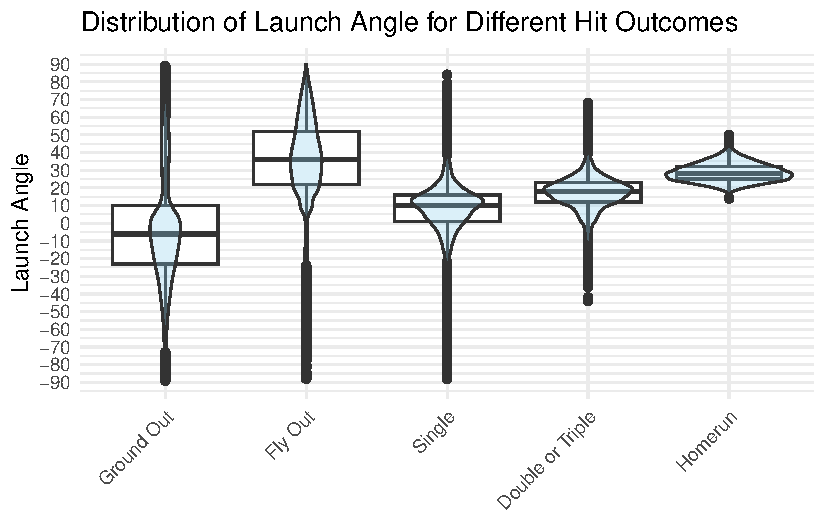
\includegraphics{V4_files/figure-pdf/fig-la-dist-1.pdf}

}

\caption{\label{fig-la-dist}Distribution and mean launch angle by hit
outcome}

\end{figure}%

Figure~\ref{fig-la-dist} shows the distribution of launch angle for
different hit outcomes. For each at bat that resulted in an actual hit
(a single, double/triple, or a homerun), it is evident that the launch
angles follow a relatively normal distribution, being unimodal and
centered around the mean. There are no drastic changes in the spread of
the data, and no discernible U-shaped pattern. Using this, the decision
to square launch angle and use a quadratic term was not made, as it is
probable that it wouldn't add much explanatory power to the model.

The side by side box plots in Figure~\ref{fig-la-dist} also indicate
that there does seem to be a difference in average launch angle for each
hit type. This supports including \texttt{launch\_angle} in the model,
and that it would be possible to have a model solely using it to predict
\texttt{hit\_outcome}, but it wouldn't explain everything. By bringing
in fly outs and ground outs, we can see how launch angle varies between
the two as well. It makes sense that the launch angle for ground outs
would tend to be lower, as it is likely that the ball was hit low on the
ground to a fielder, and the same goes for fly balls. Eventually, the
launch angle on the ball is too high and results in an out rather than a
hit. While this is the overall trend of these two specific results, the
variation and spread of the data is much larger.

It is important to note that it doesn't make sense for
\texttt{launch\_angle} to be negative for fly outs. As it is not one of
the variables that is standardized, a fly ball should have a positive
launch angle, as that would indicate that the ball went up in the air.
After examining these instances where the hit was recorded as a fly out
and the launch angle was negative, the conclusion was drawn that it was
an error in recording the data. This serves as another layer that makes
modeling this data more difficult.

\begin{figure}[H]

\centering{

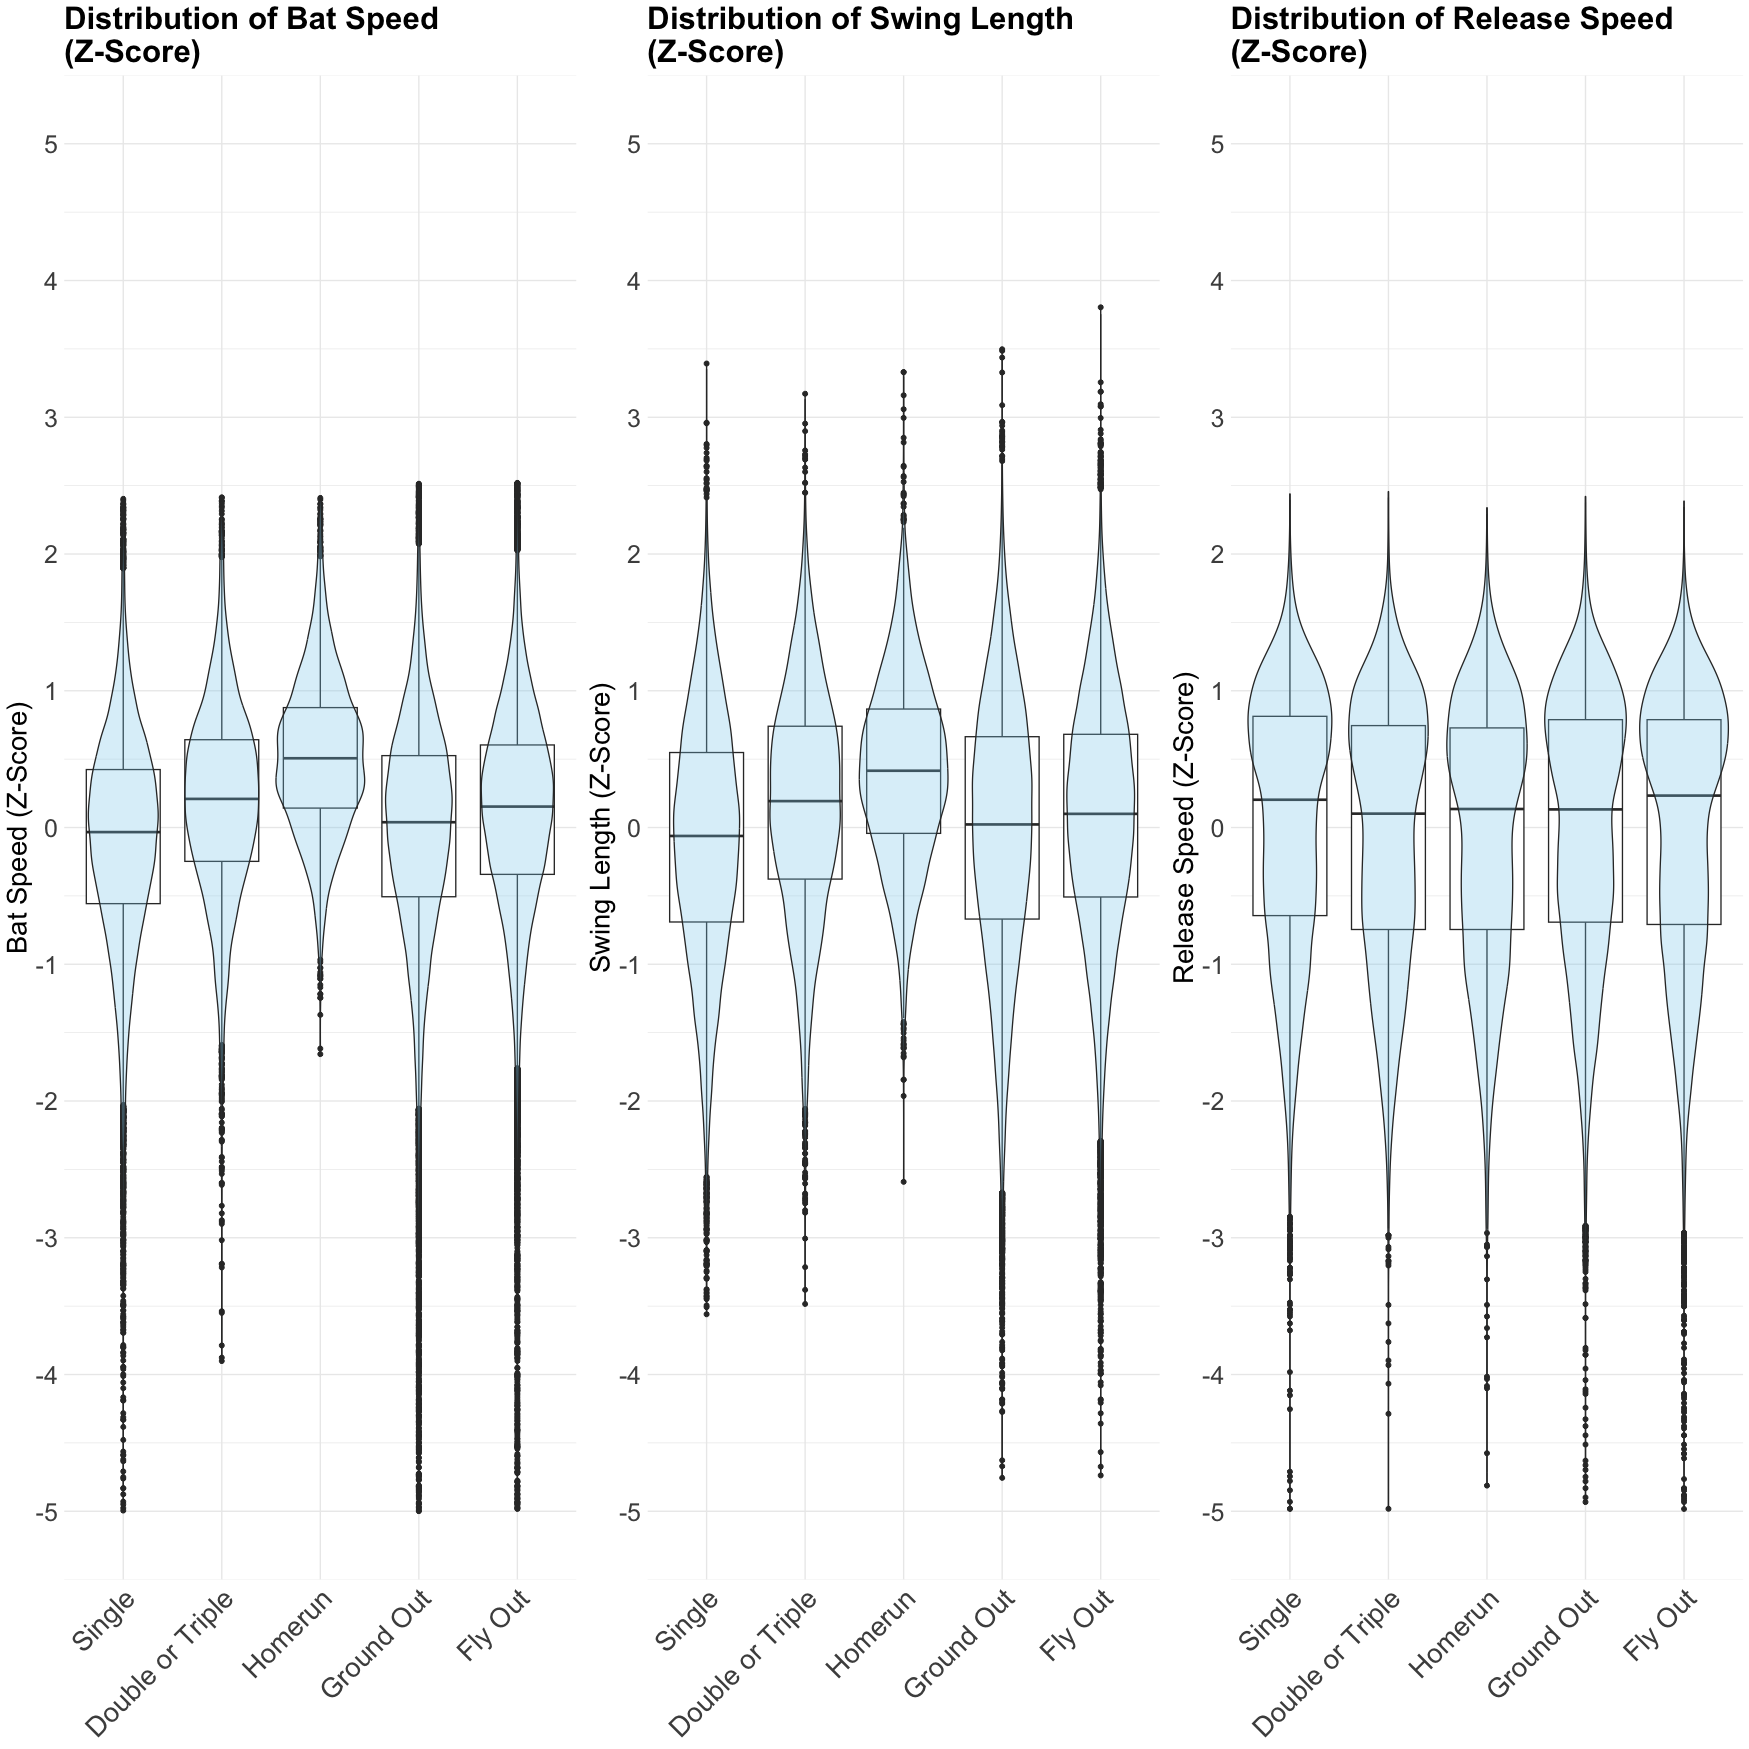
\includegraphics{combined_plots_dists.png}

}

\caption{\label{fig-dists-vars}Distributions of Dependent Variables by
Hit Outcome}

\end{figure}%

Similar to Figure~\ref{fig-la-dist}, Figure~\ref{fig-dists-vars} shows
the distribution of each standardized variable for each hit type, but
also includes fly outs and ground outs.

From these, there does seem to be differences in each variable depending
on the type of out, as well as differences in the variables depending on
the type of hit. The variable that seems the most constant is release
speed, and from that it can be drawn that the speed at which the pitch
is thrown matters less. However, release speed was still included in the
model because it aids in explaining information pertaining to the
pitcher during the at bat, and is not correlated with other variables
pertaining to the batter's mechanics.

\section{Model Development}\label{model-development}

\subsection{Stage 1}\label{stage-1}

The first stage of model development looks at simply creating logistic
regression models based on the available data. The first step of stage
one is to develop an initial model that will form the basis for the rest
of the analysis.

\subsubsection{Initial Model}\label{initial-model}

The following code describes how to make the initial multinomial
regression model, where our goal is to predict \texttt{hit\_outcome}
from \texttt{swing\_length\_zscore}, \texttt{bat\_speed\_zscore},
\texttt{release\_speed\_zscore}, \texttt{launch\_angle}, and an
interaction between \texttt{bat\_speed\_zscore} and
\texttt{swing\_length\_zscore}.

\begin{Shaded}
\begin{Highlighting}[]
\NormalTok{reg\_model\_1 }\OtherTok{\textless{}{-}} \FunctionTok{multinom}\NormalTok{(hit\_outcome }\SpecialCharTok{\textasciitilde{}} 
\NormalTok{                     swing\_length\_zscore }\SpecialCharTok{+}
\NormalTok{                     bat\_speed\_zscore }\SpecialCharTok{+}
\NormalTok{                     release\_speed\_zscore }\SpecialCharTok{+}
\NormalTok{                     launch\_angle }\SpecialCharTok{+}
\NormalTok{                     bat\_speed\_zscore}\SpecialCharTok{:}\NormalTok{swing\_length\_zscore,}
                   \AttributeTok{data =}\NormalTok{ batting\_without\_g3) }
\end{Highlighting}
\end{Shaded}

\begin{table}

\caption{\label{tbl-reg-1-output}Stage 1 Multinomial Logistic Regression
Output for Initial Model}

\centering{

\centering
\begin{tabular}[t]{l>{\raggedleft\arraybackslash}p{3cm}r>{\raggedleft\arraybackslash}p{2cm}r}
\toprule
\multicolumn{1}{c}{ } & \multicolumn{2}{c}{Double/Triple} & \multicolumn{2}{c}{Homerun} \\
\cmidrule(l{3pt}r{3pt}){2-3} \cmidrule(l{3pt}r{3pt}){4-5}
Term & Estimate  & Std. Error  & Estimate & Std. Error\\
\midrule
\cellcolor{gray!10}{Constant} & \textbf{\cellcolor{gray!10}{-1.995}} & \cellcolor{gray!10}{0.026} & \textbf{\cellcolor{gray!10}{-6.086}} & \cellcolor{gray!10}{0.072}\\
Swing Length Z-Score & \textbf{0.158} & 0.019 & \textbf{0.394} & 0.031\\
\cellcolor{gray!10}{Bat Speed Z-Score} & \textbf{\cellcolor{gray!10}{0.482}} & \cellcolor{gray!10}{0.022} & \textbf{\cellcolor{gray!10}{1.609}} & \cellcolor{gray!10}{0.038}\\
Release Speed Z-Score & -0.010 & 0.015 & \textbf{0.086} & 0.022\\
\cellcolor{gray!10}{Launch Angle} & \textbf{\cellcolor{gray!10}{0.065}} & \cellcolor{gray!10}{0.001} & \textbf{\cellcolor{gray!10}{0.208}} & \cellcolor{gray!10}{0.003}\\
\addlinespace
Swing Length/Bat Speed Interaction & \textbf{0.090} & 0.019 & \textbf{-0.243} & 0.037\\
\bottomrule
\end{tabular}

}

\end{table}%

\begin{table}

\caption{\label{tbl-reg-1-emmeans}Stage 1 emmeans Summary for Initial
Model}

\centering{

\centering
\begin{tabular}[t]{lrr}
\toprule
Hit Outcome & Average Probability & SE\\
\midrule
\cellcolor{gray!10}{1} & \cellcolor{gray!10}{0.7521163} & \cellcolor{gray!10}{0.0028169}\\
2 & 0.2264192 & 0.0027123\\
\cellcolor{gray!10}{3} & \cellcolor{gray!10}{0.0214645} & \cellcolor{gray!10}{0.0008994}\\
\bottomrule
\end{tabular}

}

\end{table}%

Table~\ref{tbl-reg-1-output} shows the multinomial regression output for
the initial model. The bold coefficients represent those that have a
p-value that is significant at the 0.01 level. Using this table, we can
view the coefficients for the model and understand how each contribute
to the hit outcome. There are two columns for the regression table, and
the coefficients in each column represent the difference in log-odds
resulting from a one unit change in the predictor between the base
group, (hitting a single) and the corresponding hit column, which can be
transformed into a probability.

For example, \texttt{launch\_angle} has a value of \(0.065\) in the
double/triple column. We can interpret this as follows:

\textbf{\emph{On average, a one degree increase in a batter's launch
angle is associated with an increase in the probability of hitting a
double or a triple by about 1.07\%}}

We can also interpret the interaction between swing length and bat
speed. With a logit coefficient of 0.09, we can turn it into a
probability and understand it as:

\textbf{\emph{The interaction between bat speed and swing length
suggests that as both increase, the likelihood of hitting a double or
triple increases compared to a single. This is reflected in the positive
interaction term, indicating that the effect of swing length on the hit
outcome is enhanced as bat speed increases.}}

The package \texttt{emmeans} in r compares the estimated marginal means.
In this model, it allows us to see the differences in the mean predicted
probabilities for each hit outcome.

Table~\ref{tbl-reg-1-emmeans} shows the estimated probabilities for each
hit outcome in this model. Singles are estimated to occur the most,
about 75.2\% of the time, followed by doubles and triples (22.6\%), and
the least likely to occur are home runs (2.1\%). While hitting a single
in a baseball game is more common than other types of hits, there is
still a stark difference in the probability of each hit occurring, this
is likely due to the imbalance in the data set, with the model being
more tailored to predicting singles because they are much more prevalent
in the data.

\paragraph{Decision Tree Initial
Model}\label{decision-tree-initial-model}

\begin{Shaded}
\begin{Highlighting}[]
\NormalTok{initial\_decision\_tree }\OtherTok{\textless{}{-}} \FunctionTok{rpart}\NormalTok{(hit\_outcome }\SpecialCharTok{\textasciitilde{}} 
\NormalTok{                                 swing\_length\_zscore }\SpecialCharTok{+}
\NormalTok{                                 bat\_speed\_zscore }\SpecialCharTok{+}
\NormalTok{                                 release\_speed\_zscore }\SpecialCharTok{+}
\NormalTok{                                 launch\_angle,}
                               \AttributeTok{data =}\NormalTok{ batting\_without\_g3,}
                               \AttributeTok{method =} \StringTok{"class"}\NormalTok{)}
\end{Highlighting}
\end{Shaded}

\begin{figure}[H]

\centering{

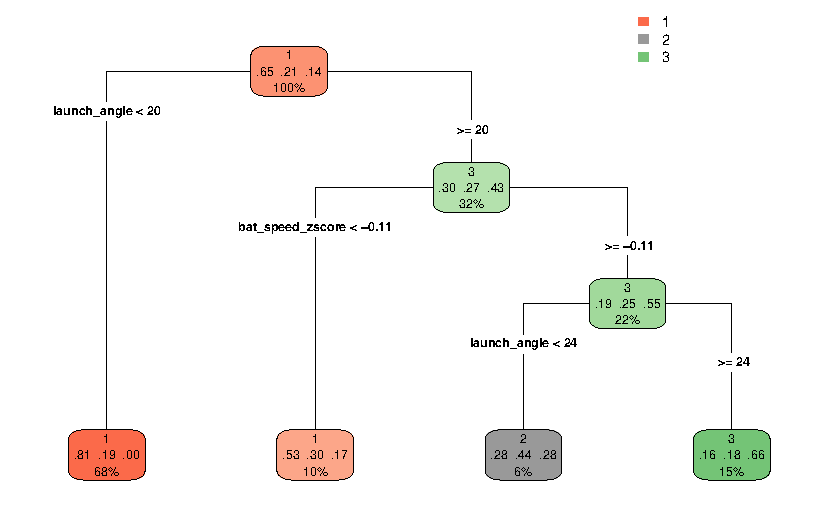
\includegraphics{V4_files/figure-pdf/fig-init-dec-tree-1.pdf}

}

\caption{\label{fig-init-dec-tree}Decision Tree for Initial Model}

\end{figure}%

Figure~\ref{fig-init-dec-tree} shows a decision tree of the initial
model. The decision tree is a classification model that visualizes the
steps that the model goes through when attempting to classify each
observation. The nodes of the tree correspond to the decisions are made
based on certain thresholds or levels of the predictor variables. The
branches represent the outcome of the decision, or the comparison that
was made, and the leaves represent the final predicted outcome of the
response variable.

From Figure~\ref{fig-init-dec-tree}, we can see that classifying the
type of hit mostly relies on a hit's launch angle and bat speed. The
model starts with all of the observations, and if the launch angle is
less than 20, the hit is automatically classified as a single. Of those
hits, it represents 68\% of the data, and of that, 81\% were actually
singles, 19\% were actually doubles/triples, and 0\% were actually
homeruns. The model continues to make similar comparisons until all
terminal nodes are reached.

Figure~\ref{fig-init-dec-tree} has four terminal nodes.
Table~\ref{tbl-decinitial-class} shows the breakdown of each terminal
node. It shows the outcome the model predicted, the percentage of the
overall observations it makes up, as well as the percent of those
observations that were actually of other classes.

\begin{table}

\caption{\label{tbl-decinitial-class}Results of stage 1 decision tree
classification for the initial model}

\centering{

\centering
\begin{tabular}[t]{lllll}
\toprule
Hit Outcome & \% Observations & \% Singles & \% Double Triple & \% Homerun\\
\midrule
\cellcolor{gray!10}{1} & \cellcolor{gray!10}{68} & \cellcolor{gray!10}{81} & \cellcolor{gray!10}{19} & \cellcolor{gray!10}{0}\\
1 & 10 & 53 & 30 & 17\\
\cellcolor{gray!10}{2} & \cellcolor{gray!10}{6} & \cellcolor{gray!10}{28} & \cellcolor{gray!10}{44} & \cellcolor{gray!10}{28}\\
3 & 15 & 16 & 18 & 66\\
\bottomrule
\end{tabular}

}

\end{table}%

It is evident that the model over classifies singles out of the data and
doesn't classify doubles/triples very well (only 6\% are being
classified as doubles/triples). Among the terminal nodes for
doubles/triples and homeruns, there is still a large percentage of those
that are being incorrectly classified as singles.

\subsubsection{Balancing}\label{balancing}

While this model has some explanatory power, the coefficient estimators
are biased and inconsistent. This is due to the inherent class imbalance
among the different hit outcomes. Biased and inconsistent estimators are
those that skewed away from the true population average.
Table~\ref{tbl-summary-sample-size} is a table corresponding to the
relative sample sizes of each hit outcome (single, extra base, or
homerun).

\begin{table}

\caption{\label{tbl-summary-sample-size}Summary of Sample Sizes for Each
Class}

\centering{

\centering
\begin{tabular}[t]{ll}
\toprule
Hit Outcome & Sample Size\\
\midrule
\cellcolor{gray!10}{Single} & \cellcolor{gray!10}{23696}\\
Double/Triple (Extra Base Hit) & 7772\\
\cellcolor{gray!10}{Homerun} & \cellcolor{gray!10}{5085}\\
\bottomrule
\end{tabular}

}

\end{table}%

Due to the fact that the sample size within the observed data for a
single is 23696, while doubles/triples and homeruns have 7772 and 5085
observations respectively, singles are going to contribute much more to
the overall model, thus causing the imbalance and bias towards
predicting the singles hit.

The singles hit in the data set are referred to as the majority class,
meaning they have the higher sample size and at this moment contribute
more to the model than the minority classes, the extra bases and the
homeruns. Intervention is necessary at this point to combat the
imbalance class size problem.

\paragraph{Existing Literature About
Balancing}\label{existing-literature-about-balancing}

A part of this project revolves around the issue of an imbalanced data
set, the implications of it, and possible solutions. The purpose of this
section is to examine literature related to the class imbalance problem
and apply it to the model predicting \texttt{hit\_outcome}.

As seen with the current batting data, a dataset is imbalanced if
different categories are not represented equally in the data. This can
lead to bias in the prediction model and flawed performance measures
(Chawla et al. (2002)). To combat this, multiple studies have been done
with the goal to develop various ways of balancing the data. Random
under sampling is the process of using random examples from the majority
class and taking them out of the dataset without replacement. This is
done until the dataset is roughly balanced. Random over sampling, on the
other hand, is the process of randomly sampling with replacement from
the category with less observations. This is also done until the data
set is somewhat balanced. (Thammasiri et al. (2014))

The effectiveness and performance of these processes are measured by the
accuracy, the error rate, sensitivity, and specificity generated from
each model's respective confusion matrix. The confusion matrix displays
the true positives (TP) identified, false positives (FP), true negatives
(TN), and false negatives (FN) (Thammasiri et al. (2014)). These
performance measures are reliable for balanced data sets, but their
reliability decreases as more imbalance is introduced in the data set.
Thus, representing another reason as to why it's important to have
balance. With the purpose of creating a more effective method to
balancing data rather than random under or over sampling, Chawla,
Bowyer, Hall, and Kegelmeyer created the Synthetic Minority Over -
Sampling (SMOTE) algorithm, which is a combination of under sampling of
the majority class and creating synthetic observations from the minority
class (Chawla et al. (2002)). SMOTE is another way to balance the
dataset so that one class doesn't have a much larger impact on the data.
SMOTE is the process of adding artificially generated data to the
minority class, following the same distribution. This method of
oversampling takes its \(k\) nearest neighbor of the same minority class
and generates a new data observation between the \(k\) neighbors and the
observed observation. The \texttt{over\_ratio} is a parameter that
specifies when SMOTE is terminated and represents the ratio of minority
class sample size to the majority class sample size. In this case, an
\texttt{over\_ratio} of one means that now the data set is exactly
balanced, all classes have the same sample size (Chawla et al. (2002)).

SMOTE is important in improving the performance of the predictive model
because it offers more examples from the underrepresented group that
follow the distribution of the data, as opposed to random over sampling,
that takes already existing data points with no extra room for the model
to learn.

In their study comparing various types of prediction techniques for
dealing with imbalanced data, Thammasiri et al. (2014), was able to rank
the performance measures of logistic regression with oversampling,
logistic regression with under sampling, logistic regression with SMOTE,
and logistic regression with the original data. After performing 10-fold
cross validation on these different models, they found that logistic
regression using SMOTE performed better than random under sampling and
oversampling. While the original data model had high accuracy it's
important to note that it could be biased and inconsistent because of
the imbalanced class sizes.

In conclusion, this literature provides useful evidence as to why the
current batting data is flawed, and a detailed approach on how to employ
the SMOTE algorithm to balance the data with the aim of creating a model
that can better predict the \texttt{hit\_outcome} of an at bat.

\subsubsection{SMOTE Model}\label{smote-model}

In order to use the SMOTE algorithm, the data needs to be cleaned
further. The code below describes this cleaning and formatting process,
and stores the data in an object called \texttt{smote\_data}.

\begin{Shaded}
\begin{Highlighting}[]
\CommentTok{\# Cleaning the data for SMOTE function }
\NormalTok{smote\_data }\OtherTok{\textless{}{-}}\NormalTok{ batting\_without\_g3 }\SpecialCharTok{\%\textgreater{}\%}
  \FunctionTok{mutate}\NormalTok{(}
    \AttributeTok{hit\_outcome\_factor =} \FunctionTok{as.factor}\NormalTok{(hit\_outcome)}
\NormalTok{  ) }\SpecialCharTok{\%\textgreater{}\%}
  \FunctionTok{select}\NormalTok{(swing\_length\_zscore,}
\NormalTok{         bat\_speed\_zscore,}
\NormalTok{         release\_speed\_zscore,}
\NormalTok{         launch\_angle,}
\NormalTok{         hit\_outcome\_factor)}
\end{Highlighting}
\end{Shaded}

After the data is in the correct format, the SMOTE algorithm can be used
with the following code. The \texttt{over\_ratio} of 0.8 indicates a
roughly balanced data set.

\begin{Shaded}
\begin{Highlighting}[]
\CommentTok{\# running the SMOTE algorithm }
\NormalTok{balanced\_batting\_data }\OtherTok{\textless{}{-}}
  \FunctionTok{smote}\NormalTok{(}
\NormalTok{    smote\_data,}
    \StringTok{"hit\_outcome\_factor"}\NormalTok{,}
    \AttributeTok{k =} \DecValTok{5}\NormalTok{,}
    \AttributeTok{over\_ratio =} \FloatTok{0.8} \CommentTok{\# a roughly balanced data set }
\NormalTok{  )}
\end{Highlighting}
\end{Shaded}

After balancing the data set, we can now run multinomial logistic
regression the same was as the initial model, except using the SMOTE
dataset.

\begin{Shaded}
\begin{Highlighting}[]
\CommentTok{\# logistic regression with the balanced data set }
\NormalTok{reg\_model\_smote}\OtherTok{\textless{}{-}} \FunctionTok{multinom}\NormalTok{(hit\_outcome\_factor }\SpecialCharTok{\textasciitilde{}}
\NormalTok{                          swing\_length\_zscore }\SpecialCharTok{+}
\NormalTok{                          bat\_speed\_zscore }\SpecialCharTok{+}
\NormalTok{                          release\_speed\_zscore }\SpecialCharTok{+}
\NormalTok{                          launch\_angle }\SpecialCharTok{+}
\NormalTok{                          bat\_speed\_zscore}\SpecialCharTok{:}\NormalTok{swing\_length\_zscore,}
                        \AttributeTok{data =}\NormalTok{ balanced\_batting\_data)}
\end{Highlighting}
\end{Shaded}

\begin{table}

\caption{\label{tbl-reg-smote-output}Stage 1 Multinomial Logistic
Regression Output for SMOTE Model}

\centering{

\centering
\begin{tabular}[t]{l>{\raggedleft\arraybackslash}p{3cm}r>{\raggedleft\arraybackslash}p{2cm}r}
\toprule
\multicolumn{1}{c}{ } & \multicolumn{2}{c}{Double/Triple} & \multicolumn{2}{c}{Homerun} \\
\cmidrule(l{3pt}r{3pt}){2-3} \cmidrule(l{3pt}r{3pt}){4-5}
Term & Estimate  & Std. Error  & Estimate & Std. Error\\
\midrule
\cellcolor{gray!10}{Constant} & \textbf{\cellcolor{gray!10}{-1.140}} & \cellcolor{gray!10}{0.019} & \textbf{\cellcolor{gray!10}{-6.147}} & \cellcolor{gray!10}{0.055}\\
Swing Length Z-Score & \textbf{0.163} & 0.015 & \textbf{0.420} & 0.022\\
\cellcolor{gray!10}{Bat Speed Z-Score} & \textbf{\cellcolor{gray!10}{0.506}} & \cellcolor{gray!10}{0.017} & \textbf{\cellcolor{gray!10}{1.794}} & \cellcolor{gray!10}{0.028}\\
Release Speed Z-Score & -0.010 & 0.011 & \textbf{0.088} & 0.015\\
\cellcolor{gray!10}{Launch Angle} & \textbf{\cellcolor{gray!10}{0.067}} & \cellcolor{gray!10}{0.001} & \textbf{\cellcolor{gray!10}{0.262}} & \cellcolor{gray!10}{0.002}\\
\addlinespace
Swing Length/Bat Speed Interaction & \textbf{0.107} & 0.015 & \textbf{-0.305} & 0.028\\
\bottomrule
\end{tabular}

}

\end{table}%

Table~\ref{tbl-reg-smote-output} shows the multinomial regression output
for the balanced smote model. We can interpret the coefficients of the
launch angle and interaction term similarly to the interpretation for
the initial model.

\texttt{launch\_angle} has a value of \(0.067\) in the double/triple
column. We can interpret this as follows:

\textbf{\emph{On average, a one degree increase in a batter's launch
angle is associated with an increase in the probability of hitting a
double or a triple by about 1.95\%}}

With a logit coefficient of \(0.107\), we can turn it into a probability
and understand the interaction between swing length and bat speed as:

\textbf{\emph{The interaction between bat speed and swing length
suggests that as both increase, the likelihood of hitting a double or
triple increases compared to a single. This is reflected in the positive
interaction term, indicating that the effect of swing length on the hit
outcome is enhanced as bat speed increases.}}

\begin{table}

\caption{\label{tbl-emmeans-smote-output}Stage 1 emmeans Summary Output
for SMOTE Model}

\centering{

\centering
\begin{tabular}[t]{lrr}
\toprule
Hit Outcome & Average Probability & SE\\
\midrule
\cellcolor{gray!10}{1} & \cellcolor{gray!10}{0.4308485} & \cellcolor{gray!10}{0.0027574}\\
2 & 0.4677700 & 0.0027754\\
\cellcolor{gray!10}{3} & \cellcolor{gray!10}{0.1013815} & \cellcolor{gray!10}{0.0019387}\\
\bottomrule
\end{tabular}

}

\end{table}%

Table~\ref{tbl-emmeans-smote-output} shows the summary output for
estimated probabilities of each hit type for the SMOTE model using a
balanced data set. After balancing the data, it can be noted now that
there is less of a difference in what hit type would be predicted, which
should be the case if there are the same amounts of observations in each
class. While the odds of predicting a single decreased, it is better for
the overall model, as a lot of singles were being incorrectly
identified.

\paragraph{Decision Tree for SMOTE
Model}\label{decision-tree-for-smote-model}

The code below generates the decision tree for the multinomial logistic
regression using the balanced SMOTE data, which is displayed in
Figure~\ref{fig-dec-tree-smote}.

\begin{Shaded}
\begin{Highlighting}[]
\NormalTok{smote\_decision\_tree }\OtherTok{\textless{}{-}} \FunctionTok{rpart}\NormalTok{(hit\_outcome\_factor }\SpecialCharTok{\textasciitilde{}}
\NormalTok{                               swing\_length\_zscore }\SpecialCharTok{+}
\NormalTok{                               bat\_speed\_zscore }\SpecialCharTok{+}
\NormalTok{                               release\_speed\_zscore }\SpecialCharTok{+}
\NormalTok{                               launch\_angle,}
                             \AttributeTok{method =} \StringTok{"class"}\NormalTok{,}
                             \AttributeTok{data =}\NormalTok{ balanced\_batting\_data)}
\end{Highlighting}
\end{Shaded}

\begin{figure}[H]

\centering{

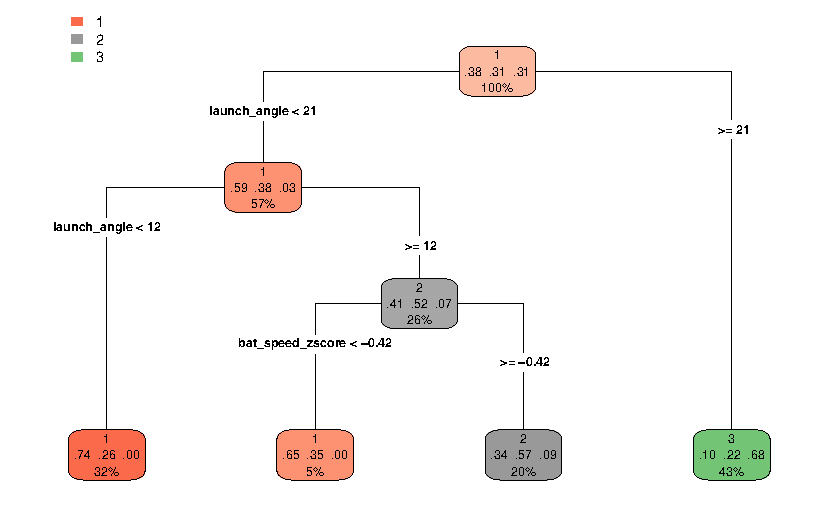
\includegraphics{V4_files/figure-pdf/fig-dec-tree-smote-1.pdf}

}

\caption{\label{fig-dec-tree-smote}Decision Tree for SMOTE Model}

\end{figure}%

Similar to the initial decision tree model, from
Figure~\ref{fig-dec-tree-smote}, we can see that classifying the type of
hit mostly relies on a hit's launch angle and bat speed. There are four
terminal nodes. Table~\ref{tbl-decsmote-class} below shows the breakdown
of each terminal node. It shows the outcome the model predicted, the
percentage of the overall observations it makes up, as well as the
percent of those observations that were actually of other classes.

\begin{table}

\caption{\label{tbl-decsmote-class}Results of stage 1 decision tree
classification for the SMOTE model}

\centering{

\centering
\begin{tabular}[t]{lllll}
\toprule
Hit Outcome & \% Observations & \% Singles & \% Double Triple & \% Homerun\\
\midrule
\cellcolor{gray!10}{1} & \cellcolor{gray!10}{32} & \cellcolor{gray!10}{74} & \cellcolor{gray!10}{26} & \cellcolor{gray!10}{0}\\
1 & 5 & 65 & 35 & 0\\
\cellcolor{gray!10}{2} & \cellcolor{gray!10}{20} & \cellcolor{gray!10}{34} & \cellcolor{gray!10}{57} & \cellcolor{gray!10}{9}\\
3 & 43 & 10 & 22 & 68\\
\bottomrule
\end{tabular}

}

\end{table}%

After balancing the data, the decision tree does a better job at
classifying doubles/triples and homeruns. In this model,57\% of the
correctly identified doubles/triples were classified correctly, opposed
to 44\% in the initial model, and the same is true for the homerun
category.

\subsection{Stage 2}\label{stage-2}

The second stage of this project examines the predicted probabilities
from the multinomial logistic regression models by feeding them into a
decision tree. In a multinomial model, the predicted probabilities
represent the likelihood that an observation belongs to a certain class.
In this case, the predicted probabilities correspond to the likelihood
that each hit is a single, double/triple, or homerun. By feeding these
predicted probabilities into a decision tree model, we're able to
identify patterns in how the probabilities map to certain classes, and
better understand the models.

\subsubsection{Initial Model}\label{initial-model-1}

Below are the steps taken to feed predicted probabilities from a
training set of the initial model into a decision tree model.

\begin{enumerate}
\def\labelenumi{\arabic{enumi}.}
\tightlist
\item
  Getting how many rows are in the data and splitting into 2 parts
\end{enumerate}

\begin{Shaded}
\begin{Highlighting}[]
\CommentTok{\# so it is reproducible}
\FunctionTok{set.seed}\NormalTok{(}\DecValTok{11}\NormalTok{)}

\CommentTok{\# number of rows in dataset }
\NormalTok{n\_batting\_initial }\OtherTok{=} \FunctionTok{nrow}\NormalTok{(batting\_without\_g3)}

\CommentTok{\# randomly take 80\% of the rows for the training object }
\NormalTok{train\_initial }\OtherTok{=} \FunctionTok{sample}\NormalTok{(}\DecValTok{1}\SpecialCharTok{:}\NormalTok{n\_batting\_initial,}
                   \FloatTok{0.8}\SpecialCharTok{*}\NormalTok{n\_batting\_initial,}
                   \AttributeTok{replace=}\ConstantTok{FALSE}\NormalTok{)}
\end{Highlighting}
\end{Shaded}

\begin{Shaded}
\begin{Highlighting}[]
\CommentTok{\# split data into two parts {-} training }
\NormalTok{batting\_train\_initial }\OtherTok{=}\NormalTok{ batting\_without\_g3[train\_initial,]}
\CommentTok{\# part that isn\textquotesingle{}t the training part}
\NormalTok{batting\_test\_initial }\OtherTok{=}\NormalTok{ batting\_without\_g3[}\SpecialCharTok{{-}}\NormalTok{train\_initial,]}
\end{Highlighting}
\end{Shaded}

\begin{enumerate}
\def\labelenumi{\arabic{enumi}.}
\setcounter{enumi}{1}
\tightlist
\item
  Getting predicted probabilities from initial model on training data
\end{enumerate}

\begin{Shaded}
\begin{Highlighting}[]
\CommentTok{\# fitting the model on the training data }
\NormalTok{reg\_train\_initial}\OtherTok{\textless{}{-}} \FunctionTok{multinom}\NormalTok{(hit\_outcome }\SpecialCharTok{\textasciitilde{}}
\NormalTok{                          swing\_length\_zscore }\SpecialCharTok{+}
\NormalTok{                          bat\_speed\_zscore }\SpecialCharTok{+}
\NormalTok{                          release\_speed\_zscore }\SpecialCharTok{+}
\NormalTok{                          launch\_angle }\SpecialCharTok{+}
\NormalTok{                          bat\_speed\_zscore}\SpecialCharTok{:}\NormalTok{swing\_length\_zscore,}
                        \AttributeTok{data =}\NormalTok{ batting\_train\_initial)}

\CommentTok{\# getting predicted probabilities }
\NormalTok{predicted\_probs\_initial }\OtherTok{\textless{}{-}} \FunctionTok{predict}\NormalTok{(reg\_train\_initial,}
                           \AttributeTok{newdata =}\NormalTok{ batting\_test\_initial,}
                           \AttributeTok{type =} \StringTok{"probs"}\NormalTok{)}

\CommentTok{\# getting predicted classes }
\NormalTok{predicted\_class\_initial }\OtherTok{\textless{}{-}} \FunctionTok{predict}\NormalTok{(reg\_train\_initial,}
                           \AttributeTok{newdata =}\NormalTok{ batting\_test\_initial,}
                           \AttributeTok{type =} \StringTok{"class"}\NormalTok{)}
\end{Highlighting}
\end{Shaded}

\begin{enumerate}
\def\labelenumi{\arabic{enumi}.}
\setcounter{enumi}{2}
\tightlist
\item
  Feeding the predicted probabilities into a decision tree
\end{enumerate}

\begin{Shaded}
\begin{Highlighting}[]
\NormalTok{stage\_2\_tree\_initial }\OtherTok{\textless{}{-}} \FunctionTok{rpart}\NormalTok{(hit\_outcome }\SpecialCharTok{\textasciitilde{}}
\NormalTok{                        predicted\_probs\_initial,}
                      \AttributeTok{method =} \StringTok{"class"}\NormalTok{,}
                      \AttributeTok{data =}\NormalTok{ batting\_test\_initial)}
\end{Highlighting}
\end{Shaded}

\begin{figure}[H]

\centering{

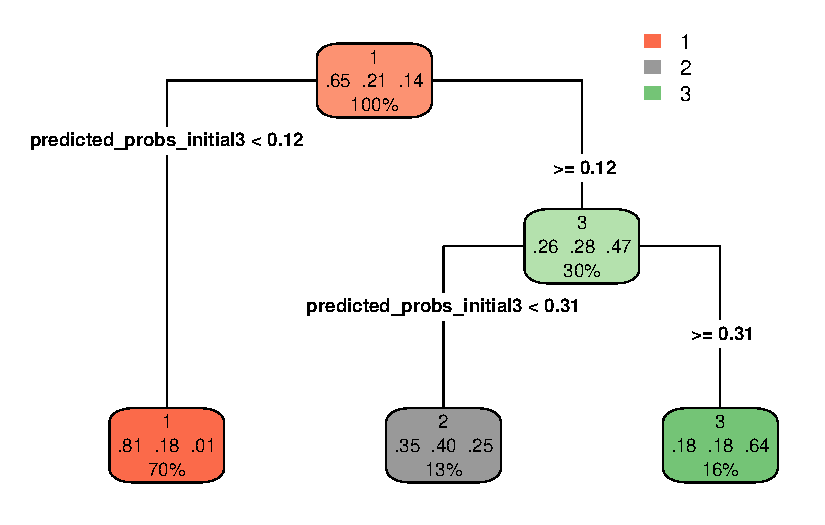
\includegraphics{V4_files/figure-pdf/fig-init-pred-dectree-1.pdf}

}

\caption{\label{fig-init-pred-dectree}Stage 2 Decision Tree from
Predicted Probabilities (Initial Model)}

\end{figure}%

Figure~\ref{fig-init-pred-dectree} Shows the how the predicted
probabilities affect the overall classification of the observation.
\texttt{predicted\_probs\_initial\_tree3} represents the predicted
probability that the observation is a homerun. We can see that the model
is only using that predicted probability to classify the hits. If that
probability is less than 0.12, it is automatically classified as a
single. If it's more than 0.12, it is compared again, this time to 0.31.
Any hit with a predicted probability less than 0.31 is classified as a
double/triple, and a probability greater than that is classified as a
homerun. The summary table below shows the percentages for each terminal
node.

\begin{figure}[H]

\centering{

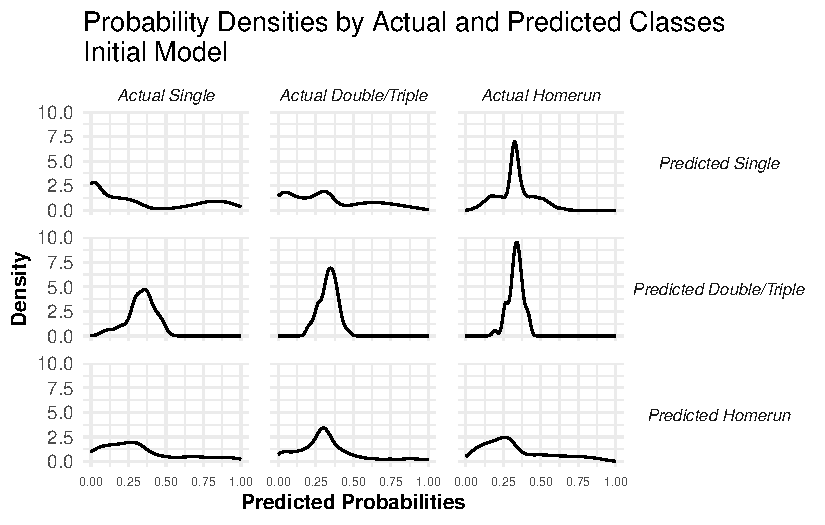
\includegraphics{V4_files/figure-pdf/fig-prob-den-initial-1.pdf}

}

\caption{\label{fig-prob-den-initial}Comparing the probability
distributions across combinations of actual vs.~predicted hits for the
initial model}

\end{figure}%

Figure~\ref{fig-prob-den-initial} shows each of the density
distributions for the observations based on their predicted and actual
class. By following a specific column and row of the graph, you can look
at combinations of hits and the different predicted probabilities that
were generated by the model. The diagonal line of three graphs going
through the center correspond to hits that were correctly classified,
while the distributions around the diagonal line were incorrectly
classified.

We can see from Figure~\ref{fig-prob-den-initial} that for hits that
were actually doubles/triples and were correctly classified as
doubles/triples, there is a high concentration of predicted
probabilities ranging from 0.25-0.5, with a peak being around 0.35. This
means that for hits that were correctly classified as doubles/triples in
the initial model were all done so with less than 50\% certainty. This
graph can be used to understand the ability of the model to be confident
in certain classifications.

\subsubsection{SMOTE Model}\label{smote-model-1}

A similar process was done to the data used for the SMOTE model in order
to create a decision tree from the predicted probabilities based on that
data.

\begin{enumerate}
\def\labelenumi{\arabic{enumi}.}
\tightlist
\item
  Getting how many rows are in the data and splitting into 2 parts
\end{enumerate}

\begin{Shaded}
\begin{Highlighting}[]
\CommentTok{\# reproducibility }
\FunctionTok{set.seed}\NormalTok{(}\DecValTok{11}\NormalTok{)}

\CommentTok{\# number of rows }
\NormalTok{n\_batting\_smote }\OtherTok{=} \FunctionTok{nrow}\NormalTok{(balanced\_batting\_data)}

\CommentTok{\# randomly take 80\% of the rows for the training object }
\NormalTok{train\_smote }\OtherTok{=} \FunctionTok{sample}\NormalTok{(}\DecValTok{1}\SpecialCharTok{:}\NormalTok{n\_batting\_smote,}
                     \FloatTok{0.8}\SpecialCharTok{*}\NormalTok{n\_batting\_smote,}
                     \AttributeTok{replace=}\ConstantTok{FALSE}\NormalTok{)}
\end{Highlighting}
\end{Shaded}

\begin{Shaded}
\begin{Highlighting}[]
\CommentTok{\# split data into two parts}
\NormalTok{batting\_train\_smote }\OtherTok{=}\NormalTok{ balanced\_batting\_data[train\_smote,]}
\CommentTok{\# part that isn\textquotesingle{}t the training part}
\NormalTok{batting\_test\_smote }\OtherTok{=}\NormalTok{ balanced\_batting\_data[}\SpecialCharTok{{-}}\NormalTok{train\_smote,]}
\end{Highlighting}
\end{Shaded}

\begin{enumerate}
\def\labelenumi{\arabic{enumi}.}
\setcounter{enumi}{1}
\tightlist
\item
  Getting Predicted Probabilities from SMOTE Model on training data
\end{enumerate}

\begin{Shaded}
\begin{Highlighting}[]
\CommentTok{\# fitting the model on the training data }
\NormalTok{reg\_train\_smote }\OtherTok{\textless{}{-}} \FunctionTok{multinom}\NormalTok{(hit\_outcome\_factor }\SpecialCharTok{\textasciitilde{}}
\NormalTok{                          swing\_length\_zscore }\SpecialCharTok{+}
\NormalTok{                          bat\_speed\_zscore }\SpecialCharTok{+}
\NormalTok{                          release\_speed\_zscore }\SpecialCharTok{+}
\NormalTok{                          launch\_angle }\SpecialCharTok{+}
\NormalTok{                          bat\_speed\_zscore}\SpecialCharTok{:}\NormalTok{swing\_length\_zscore,}
                        \AttributeTok{data =}\NormalTok{ batting\_train\_smote)}

\CommentTok{\# getting predicted probabilities }
\NormalTok{predicted\_probs\_smote }\OtherTok{\textless{}{-}} \FunctionTok{predict}\NormalTok{(reg\_train\_smote,}
                                 \AttributeTok{newdata =}\NormalTok{ batting\_test\_smote,}
                                 \AttributeTok{type =} \StringTok{"probs"}\NormalTok{)}

\CommentTok{\# getting predicted classes }
\NormalTok{predicted\_class\_smote }\OtherTok{\textless{}{-}} \FunctionTok{predict}\NormalTok{(reg\_train\_smote,}
                                      \AttributeTok{newdata =}\NormalTok{ batting\_test\_smote,}
                                      \AttributeTok{type =} \StringTok{"class"}\NormalTok{)}
\end{Highlighting}
\end{Shaded}

\begin{enumerate}
\def\labelenumi{\arabic{enumi}.}
\setcounter{enumi}{2}
\tightlist
\item
  Feeding into decision tree the predicted probabilities
\end{enumerate}

\begin{Shaded}
\begin{Highlighting}[]
\NormalTok{stage\_2\_tree\_smote }\OtherTok{\textless{}{-}} \FunctionTok{rpart}\NormalTok{(hit\_outcome\_factor }\SpecialCharTok{\textasciitilde{}}
\NormalTok{                              predicted\_probs\_smote,}
                            \AttributeTok{method =} \StringTok{"class"}\NormalTok{,}
                            \AttributeTok{data =}\NormalTok{ batting\_test\_smote)}
\end{Highlighting}
\end{Shaded}

\begin{figure}[H]

\centering{

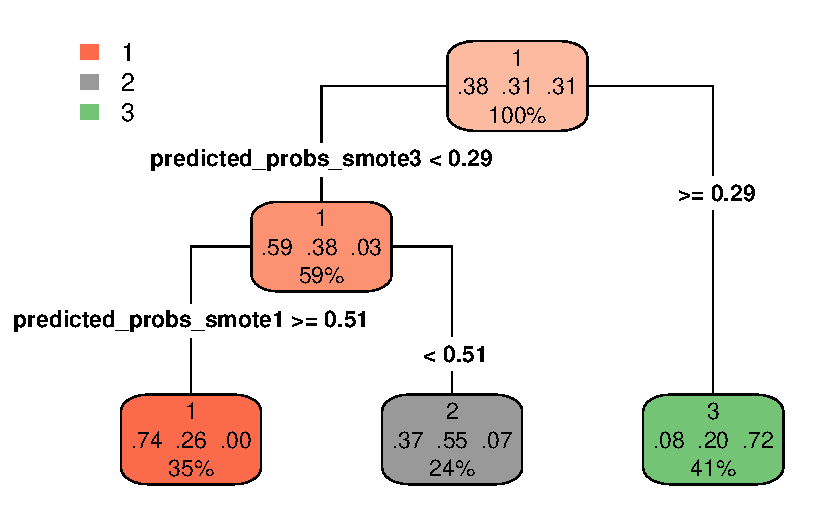
\includegraphics{V4_files/figure-pdf/fig-smote-pred-dectree-1.pdf}

}

\caption{\label{fig-smote-pred-dectree}Decision Tree from Predicted
Probabilities (SMOTE Model)}

\end{figure}%

Figure~\ref{fig-smote-pred-dectree} shows the decision tree trained from
the predicted probabilities of the balanced SMOTE model. The model
begins by looking at if the predicted probability of the hit being a
homerun (\texttt{predicted\_probs\_smote3} \textless{} 0.29). If that
probability is greater than or equal to 0.29, it is classified as a
homerun. If it is less than 0.29, the model looks at the predicted
probability being a single. If that predicted probability is greater
than 0.51 the observation is classified as a single, if not, a
double/triple. This model first attempts to determine if a hit is a
homerun or not, and then tries to separate the singles from the
doubles/triples. This strategy differs from the initial model, which
first decided if a hit was a single and then compared the other types.

\begin{figure}[H]

\centering{

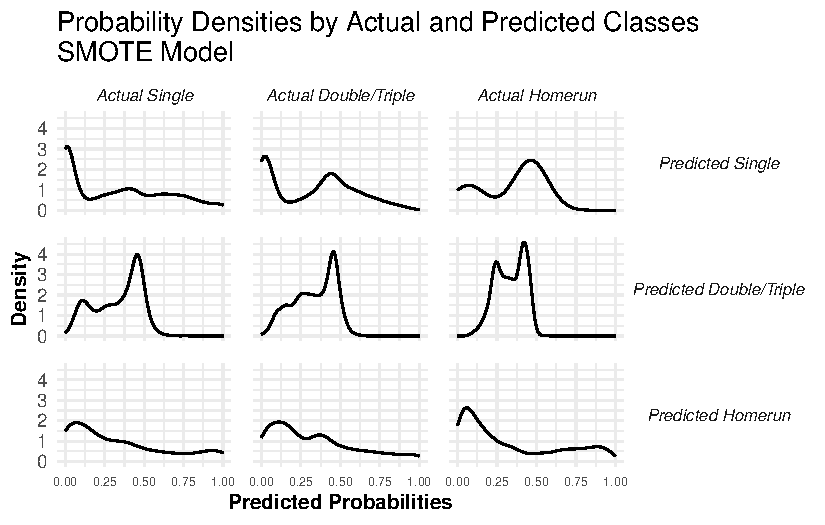
\includegraphics{V4_files/figure-pdf/fig-pred-den-smote-1.pdf}

}

\caption{\label{fig-pred-den-smote}Comparing the probability
distributions across combinations of actual vs.~predicted hits for the
smote model}

\end{figure}%

Figure~\ref{fig-pred-den-smote} shows the density graphs of the
predicted probabilities for the SMOTE model. The density distributions
of hits that were incorrectly classified tended to smooth out. However
there are still some instances where the model is consistently wrong.
The model does a poor job at distinguishing between a single and
doubles/triples. This is evident by the graphs where singles and
doubles/triples were misclassified as the other. For example, the
observations that were actually singles but were classified as
doubles/triples has a high density of predicted probabilities around
0.5, meaning that the model was getting a high probability of the hit
being a double/triple when it was actually a single for the majority of
hits that fall in that category.

\section{Model Evaluation}\label{model-evaluation}

The initial model attempts to classify the hit type using the
standardized swing length, standardized bat speed, standardized release
speed, launch angle, and an interaction between standardized bat speed
and standardized swing length. All predictors in the model are
significant and bat speed and swing length seem to contribute the most
to model.

The SMOTE model takes all of the same predictors, but uses different
data. The new balanced data has roughly the same amount of observations
among classes to prevent one class from creating bias. All predictors in
this model are significant and bat speed and swing length both
contribute the most to the model as well.

\subsection{Confusion Matrix Initial
Model}\label{confusion-matrix-initial-model}

\begin{figure}[H]

\centering{

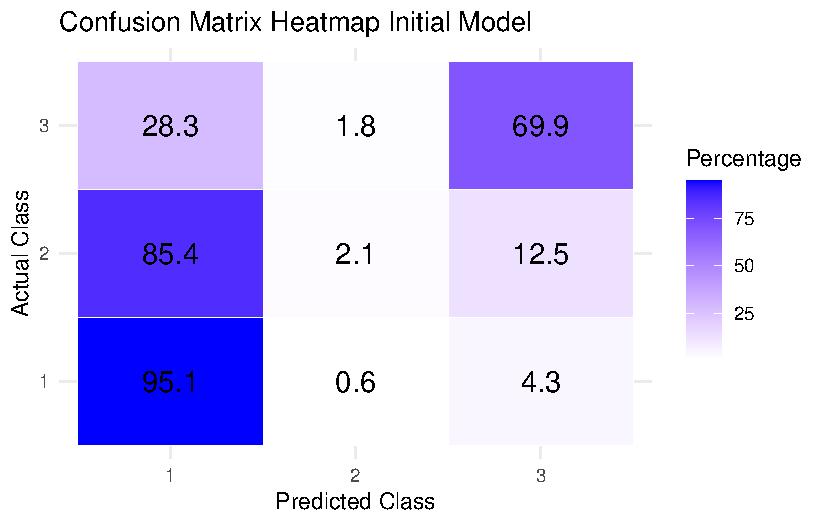
\includegraphics{V4_files/figure-pdf/fig-confusion-initial-1.pdf}

}

\caption{\label{fig-confusion-initial}Confusion Matrix for Initial Model
showing the percentage of the actual class that was classified to the
corresponding category}

\end{figure}%

Figure~\ref{fig-confusion-initial} shows the confusion matrix for the
initial multinomial logistic regression model. The percentages in each
box indicate the percent of the total number of hits in that class the
prediction makes up. For example, 95.1\% of the observed singles were
correctly identified as singles, while 2.1\% of the observed
doubles/triples were correctly identified as doubles/triples and 69.9\%
of homeruns were correctly classified as homerun. We can also use this
confusion matrix to find weak spots in the model. For example, 85.4\% of
all hits that were actually doubles/triples were classified as singles,
and 28.3\% of homeruns were classified as singles.

Figure~\ref{fig-confusion-initial} provides evidence for the fact that
because the initial data set is so imbalanced, the model incorrectly
identifies singles at higher rates than any other hit. This is seen as
the darkest colors, indicating high percentages, and more concentrated
in the predicted singles column, and the percentages get lower
everywhere else.

From the numbers behind the percentages of
Figure~\ref{fig-confusion-initial}, we can find the accuracy as:

\[ Accuracy = \frac{TP + TN}{TP + FP + TN + FN} = \frac{22536 + 166 + 3552}{36553} = 0.7182\]

While accuracy is a respected metric for evaluating model performance,
it should not be the only one evaluated in a multinomial classification
model. This is because accuracy fails to take into account the number of
correctly identified observations of the other classes. It also fails to
account for class balance. For these reasons, it is also important to
look at precision for a certain level, \(i\)

\[Precision_{singles} = \frac{22536}{22536 + 6635+ 1441} = 0.736\]
\[Precision_{extraBH} = \frac{166}{166 + 139 + 92} = 0.418\]
\[Precision_{HomeRuns} = \frac{3552}{3552 + 971 + 1021} = 0.641\]

As the precision measures indicate, the model is not precise at all in
predicting extra base hits and homeruns, and that the majority of the
accuracy comes from predicting singles.

\subsection{Confusion Matrix SMOTE
Model}\label{confusion-matrix-smote-model}

\begin{figure}[H]

\centering{

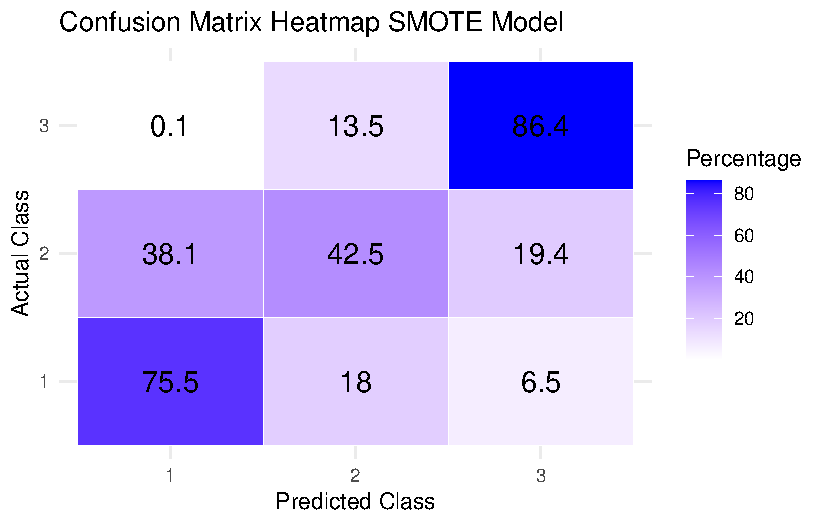
\includegraphics[width=0.85\textwidth,height=0.85\textheight]{V4_files/figure-pdf/fig-confusion-smote-1.pdf}

}

\caption{\label{fig-confusion-smote}Confusion matrix for SMOTE model
showing the percentage of the actual class that was classified in that
category}

\end{figure}%

\[ Accuracy = \frac{17899 + 8082 + 16350}{61608} = 0.6871\]
\[Precision_{singles} = \frac{17899}{17899 + 7196 + 21} = 0.713\]
\[Precision_{extraBH} = \frac{8082}{8082 + 4249 + 2585} = 0.542\]
\[Precision_{HomeRuns} = \frac{16350}{16350 + 3678 + 1548} = 0.758\]

Figure~\ref{fig-confusion-smote} shows how with the balanced data set,
the model does a better job at predicting hits that aren't singles.
While the percent of singles that were correctly predicted declines, the
trade off is a much higher rate of doubles/triples that were correctly
predicted, as well as home runs. This is also evident in the precision
calculations for each level of the hit outcome. While the overall
accuracy of the model declines, we can see that the precision for the
extra base hits and homeruns are significantly higher compared to the
initial model.

\section{Discussion and Implications}\label{discussion-and-implications}

\begin{table}

\caption{\label{tbl-acc-prec-comp}Accuracy and Precision Comparison}

\centering{

\centering
\begin{tabular}[t]{lllll}
\toprule
Model & Accuracy & Precision S & Precision Extra BH & Precision HR\\
\midrule
\cellcolor{gray!10}{Initial} & \cellcolor{gray!10}{0.7182} & \cellcolor{gray!10}{0.736} & \cellcolor{gray!10}{0.418} & \cellcolor{gray!10}{0.641}\\
SMOTE & 0.6871 & 0.713 & 0.542 & 0.758\\
\bottomrule
\end{tabular}

}

\end{table}%

Table~\ref{tbl-acc-prec-comp} shows side by side comparisons of accuracy
and precision for each model. While the models aren't perfect and there
are inherent issues with class balance, bias, accuracy, and precision,
the SMOTE model using synthetic data does a better job than the initial
model according to these metrics. There are still issues with
classification, as seen in the predicted probabilities. The SMOTE model
is not extremely accurate in distinguishing singles from
doubles/triples, but does a better job than the initial one. This
iniability could simply be from the wide variation in ways a batter can
hit a single, double/triple, which makes modeling difficult.

\newpage

\section*{References}\label{references}
\addcontentsline{toc}{section}{References}

\phantomsection\label{refs}
\begin{CSLReferences}{1}{0}
\bibitem[\citeproctext]{ref-chawla2002smote}
Chawla, Nitesh V, Kevin W Bowyer, Lawrence O Hall, and W Philip
Kegelmeyer. 2002. {``SMOTE: Synthetic Minority over-Sampling
Technique.''} \emph{Journal of Artificial Intelligence Research} 16:
321--57.

\bibitem[\citeproctext]{ref-baseballr}
Petti, Bill, and Saiem Gilani. 2024. \emph{Baseballr: Acquiring and
Analyzing Baseball Data}. \url{https://github.com/mlascaleia/baseballr}.

\bibitem[\citeproctext]{ref-baseballsavant}
Statcast, MLB. 2024. {``Statcast Bat Tracking Leaderboard.''} Major
League Baseball.
\url{https://baseballsavant.mlb.com/leaderboard/bat-tracking}.

\bibitem[\citeproctext]{ref-thammasiri2014critical}
Thammasiri, Dech, Dursun Delen, Phayung Meesad, and Nihat Kasap. 2014.
{``A Critical Assessment of Imbalanced Class Distribution Problem: The
Case of Predicting Freshmen Student Attrition.''} \emph{Expert Systems
with Applications} 41 (2): 321--30.

\bibitem[\citeproctext]{ref-wu2012cluster}
Wu, Junjie, and Junjie Wu. 2012. {``Cluster Analysis and k-Means
Clustering: An Introduction.''} \emph{Advances in K-Means Clustering: A
Data Mining Thinking}, 1--16.

\end{CSLReferences}



\end{document}
